% !TeX root = ../../thesis.tex

\setcounter{equation}{0}
\chapter{Theoretical Framework and
Methods} \label{sec:Background}

This thesis examines how yielding and fracture emerge in simplified theoretical models of soft disordered solids, with particular emphasis on disordered networks. The central problem is to understand how bulk mechanical response is connected to local damage, rearrangement, and eventual loss of load-bearing capacity.

A key difficulty is the separation of scales involved in failure. Stress and strain are imposed and measured at the continuum level, but yielding and fracture originate through local rearrangements and bond-scale damage. Continuum variables are therefore needed to describe loading, force balance, and macroscopic response \cite{chandrasekharaiahContinuumMechanics2014,lubliner2008plasticity,macoskoRheologyPrinciplesMeasurements1994}, but they do not by themselves identify where damage begins or how it redistributes stress through a heterogeneous structure.

For this reason, the chapter moves from continuum mechanics to mesoscopic and discrete descriptions. We first introduce the rheological variables and overdamped force-balance framework used throughout the thesis. We then turn to models in which local rearrangements, stress relaxation, and bond failure can be resolved explicitly \cite{falk_dynamics_1998,maloney_amorphous_2006,tanguy_plastic_2006,gartner_nonlinear_2016,picard_elastic_2004}. This leads naturally to disordered lattice and filament-network models, which provide a minimal setting for studying damage accumulation, stress redistribution, and fracture in heterogeneous solids \cite{mackintosh_elasticity_1995,storm_nonlinear_2005,broedersz_modeling_2014,broedersz_criticality_2011,feng_nonlinear_2016,tauber_stretchy_2022}.

\section{Introduction to Rheology} \label{sec:IntroRheology}

Rheology is the study of how materials respond to applied stress, relating stress to the resulting deformation or rate of deformation \cite{larson_structure_1999,chenRheologySoftMaterials2010,tannerEngineeringRheology2000,barnes_introduction_1989}. The term originates from the early 20th century and comes from the Greek words \quotes{rheo}, meaning \quotes{to flow}, and \quotes{logos}, meaning \quotes{study} \cite{barnes_introduction_1989}. Early work by Hooke \cite{hooke_lectures_1678} and Newton \cite{newton_philosophiae_1687} established the simplest linear relations between stress and strain, and between stress and strain rate. Modern rheology, however, is primarily concerned with materials for which these simple linear relations break down and non-linear behaviour governs the response. Since the later chapters focus on such regimes, we introduce here only the concepts of stress and strain needed for the remainder of the thesis. The aim is not to provide a complete treatment of rheology, but rather a concise framework for interpreting the results that follow; for a fuller account, the reader is referred to the standard texts cited throughout this chapter.

\subsection{Stress and Strain} \label{sec:StressAndStrain}

The concepts of stress and strain form the basis of rheology. Strain quantifies the deformation of a material, while stress measures the internal forces that arise in response to that deformation.

The simplest measure of strain is the relative change in length,
\begin{equation}
    \epsilon = \frac{\Delta x}{L},
    \label{eq:simpleStrain}
\end{equation}
where $\Delta x$ is the change in length and $L$ is the original length measured along the same axis \cite{lubliner2008plasticity,macoskoRheologyPrinciplesMeasurements1994,barnes_introduction_1989}. This definition corresponds to extensional (or normal) deformation, in which a material element changes its length along a given direction. In contrast, materials may also deform through shear, in which layers of material slide past one another without a change in volume. In simple shear, if the upper boundary of a material is displaced by $\Delta x$ over a separation $L_y$, the shear strain is defined as
\begin{equation}
    \gamma_{xy} = \frac{\Delta x}{L_y}.
\end{equation}
\cite{lubliner2008plasticity,macoskoRheologyPrinciplesMeasurements1994,barnes_introduction_1989} These two fundamental modes of deformation are illustrated in \cref{fig:typesOfStrain}.

Extension and shear represent the fundamental forms of deformation, with more general deformations arising as combinations of the two. Since both $\epsilon$ and $\gamma_{xy}$ are defined relative to the undeformed configuration, they correspond to engineering strains, and the term strain will be used in this sense unless otherwise specified.

\begin{figure}
    \centering
    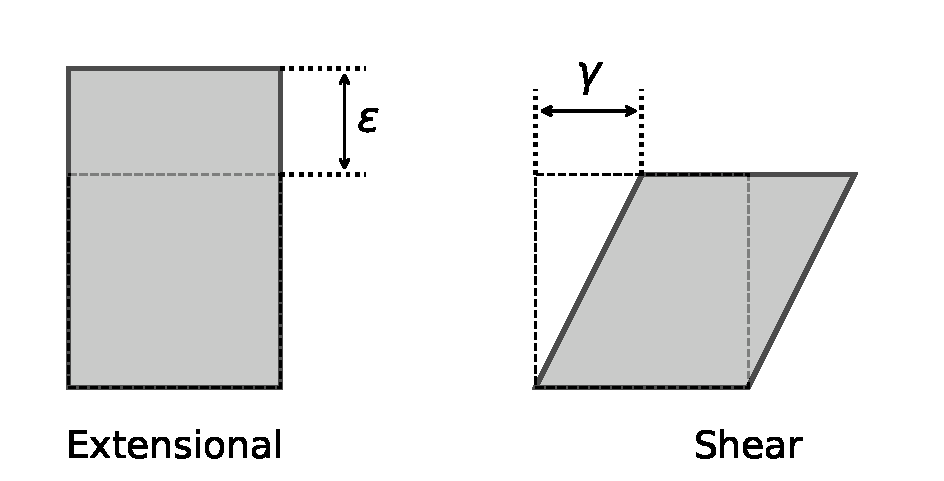
\includegraphics[width=.95\linewidth]{chapters/2-Background/Figures/StrainModes.pdf}
    \caption[Illustration of the two fundamental strain modes in 2D]{Illustration of the two fundamental strain modes in 2D: extensional strain ($\epsilon$), where the element changes length, and shear strain ($\gamma$), where the element changes shape through angular distortion. The dashed lines denote the material's undeformed configuration, while the solid lines indicate its deformed state.}
    \label{fig:typesOfStrain}
\end{figure}

Correspondingly, stress may be defined as the force per unit area transmitted across a surface,
\begin{equation}
    \sigma = \frac{F}{A},
    \label{eq:simpleStress}
\end{equation}
where $F$ is the force acting on an area $A$ \cite{,macoskoRheologyPrinciplesMeasurements1994,barnes_introduction_1989}.

Both stress and strain are inherently directional quantities. Strain depends on the direction along which deformation is measured, while stress depends on both the orientation of the surface and the direction of the force acting across it. Consequently, they are most naturally described by second-rank tensors, the stress tensor $\bm{\sigma}$ and the strain tensor $\bm{\epsilon}$. The components of these tensors reflect the two deformation modes introduced above. Diagonal components correspond to normal stresses and extensional or compressive deformations while, off-diagonal components correspond to shear deformation and shear stresses. In \cref{sec:StrainTensor,sec:StressTensor}, we construct these tensors more formally, but we refer the reader to Refs.~\cite{tannerEngineeringRheology2000, chandrasekharaiahContinuumMechanics2014} for a more detailed treatment.

\subsection{Strain Tensor} \label{sec:StrainTensor}

The engineering strains introduced above are useful for simple extension and shear, but in general a material element may stretch, compress, and shear in different directions simultaneously. To describe such local deformations, it is convenient to work in terms of the displacement field and its gradients.

We start by considering a material point initially at position $\bm{x}$, which is displaced to a new position $\bm{X}(\bm{x})$. The resulting displacement field is defined as
\[
    \bm{u}(\bm{x}) = \bm{X}(\bm{x}) - \bm{x}.
\]

While $\bm{u}(\bm{x})$ describes the motion of an individual material point, deformation is determined by spatial variations of the displacement field. To quantify this, we consider two nearby material points separated in the reference configuration by $d\bm{x}$. Since $\bm{X}(\bm{x}) = \bm{x} + \bm{u}(\bm{x})$, the separation after the applied deformation is
\[
    d\bm{X} = \frac{\partial \bm{X}}{\partial \bm{x}} d\bm{x} = \bm{F} d\bm{x} = \left( \bm{I} + \frac{\partial \bm{u}}{\partial \bm{x}} \right) d\bm{x},
\]
where $\bm{F}$ is the deformation gradient. The corresponding change in separation is therefore
\[
    d\bm{u} = d\bm{X} - d\bm{x} = \frac{\partial \bm{u}}{\partial \bm{x}} d\bm{x},
\]
such that the local deformation is characterised by the displacement gradient $\nabla \bm{u}$ (or in components, $\partial u_i/\partial x_j$).

Since the displacement gradient contains contributions from both deformation and rigid-body rotation, it may be decomposed as 
\[
    \nabla \bm{u} = \bm{\epsilon} + \bm{\omega},
\]
where $\bm{\epsilon}$ is symmetric and $\bm{\omega}$ is antisymmetric. The antisymmetric part corresponds to bulk rigid-body rotations and does not contribute to the measured local deformation. The strain tensor, which qunatifies this local deformation, can therefore be defined as the symmetric part of the displacement gradient,
\begin{equation}
\bm{\epsilon} = \frac{1}{2}\left( \nabla \bm{u} + (\nabla \bm{u})^T \right),
\label{eq:linearStrain}
\end{equation}
where we have neglected higher-order terms in the displacement gradient, which are small in the limit of small deformations. This definition is known as the linearised strain tensor or infinitesimal strain tensor \cite{chandrasekharaiahContinuumMechanics2014}.

In Cartesian coordinates, the corresponding strain tensor in three dimensions may therefore be written as
\[
    \bm{\epsilon} =
    \begin{bmatrix}
        \dfrac{\partial u_x}{\partial x} & \dfrac{1}{2}\left( \dfrac{\partial u_x}{\partial y} + \dfrac{\partial u_y}{\partial x} \right) & \dfrac{1}{2}\left( \dfrac{\partial u_x}{\partial z} + \dfrac{\partial u_z}{\partial x} \right) \\[6pt]
        \dfrac{1}{2}\left( \dfrac{\partial u_y}{\partial x} + \dfrac{\partial u_x}{\partial y} \right) & \dfrac{\partial u_y}{\partial y} & \dfrac{1}{2}\left( \dfrac{\partial u_y}{\partial z} + \dfrac{\partial u_z}{\partial y} \right) \\[6pt]
        \dfrac{1}{2}\left( \dfrac{\partial u_z}{\partial x} + \dfrac{\partial u_x}{\partial z} \right) & \dfrac{1}{2}\left( \dfrac{\partial u_z}{\partial y} + \dfrac{\partial u_y}{\partial z} \right) & \dfrac{\partial u_z}{\partial z}
    \end{bmatrix}.
\]
The diagonal components of this tensor represent normal strains, corresponding to fractional changes in length along the $x$, $y$, and $z$ directions, while the off-diagonal components represent shear strains, corresponding to changes in the angle between material line elements. These off-diagonal components are related to the engineering shear strains introduced in \cref{sec:StressAndStrain} through
\begin{equation}
    \gamma_{ij} = 2\epsilon_{ij}, \qquad i \neq j,
    \label{eq:engineeringShearStrain}
\end{equation}
so that, for example, $\gamma_{xy} = 2\epsilon_{xy}$. Alternatively, since the strain tensor is symmetric, there exists a basis, known as the principal axes, in which the tensor is diagonal and the off-diagonal components vanish.

A further decomposition of the symmetric strain tensor $\bm{\epsilon}$ separates it into deviatoric and volumetric parts,
\[
    \bm{\epsilon} = \bm{d} + \frac{1}{D} \mathrm{Tr}(\bm{\epsilon}) \bm{I},
\]
where $\bm{d}$ is the deviatoric (traceless) part, $\bm{I}$ is the identity tensor, and $D$ is the dimensionality of the space. For incompressible materials, the volumetric strain vanishes, so that $\mathrm{Tr}(\bm{\epsilon}) = 0$ and the strain is purely deviatoric, $\bm{\epsilon} = \bm{d}$. This decomposition will be useful in the continuum descriptions developed later.

The form presented above is only valid in the limit of small deformations, where the displacement gradients are sufficiently small that higher-order terms can be neglected. For larger deformations, finite-strain measures such as the Green–Lagrange strain tensor must be used \cite{TruesdellNoll1992}. In this thesis, the linearised strain tensor serves as the common language used to discuss local elastic response, force balance, and stress redistribution.

\subsection{Stress Tensor} \label{sec:StressTensor}
We now introduce the stress tensor, which describes how internal forces are distributed through a material.

If we consider a surface element of area $A$ within a material. The force $\bm{T}$ acting across this surface defines the traction,
\begin{equation}
    \bm{s} = \lim_{A \to 0} \frac{\bm{T}}{A},
\end{equation}
which represents the force per unit area acting on a surface with a given orientation.

To characterise the internal state of stress at a point, we may imagine making an arbitary cut through the material passing through that point. The traction $\bm{s}$ then represents the force exerted across this cut. However, the form of the traction vector $\bm{s}$ depends on the orientation of the cut. Different cuts through the same point, with different normals, will in general yield different traction vectors $\bm{s}$.

A single traction vector $\bm{s}$ therefore provides only partial information about the internal state of stress. Instead, the full state of stress at a point is determined by the set of all traction vectors acting on all possible planes through that point. To relate these traction vectors, we consider an infinitesimal tetrahedral element with three faces aligned with the coordinate planes, with normals $\bm{n}^{(x)}$, $\bm{n}^{(y)}$, and $\bm{n}^{(z)}$, and a fourth inclined face with normal $\bm{n}$. Requiring force balance on this element shows that the traction $\bm{s}(\bm{n})$ acting on the inclined face can be written as a linear combination of the tractions $\bm{s}(\bm{n}^{(x)})$, $\bm{s}(\bm{n}^{(y)})$, and $\bm{s}(\bm{n}^{(z)})$ acting on the coordinate planes. In the limit as the tetrahedron shrinks to a point, the traction therefore depends linearly on the surface normal $\bm{n}$. This construction is illustrated in \cref{fig:CauchyTetrahedron}. More generally, the stress tensor may be expressed in any orthonormal basis. As described for strain, there exists a set of principal axes for which the traction vectors on the corresponding coordinate planes are parallel to the plane normals, so that the stress tensor is diagonal in this basis.

\begin{figure}[t!]
    \centering
    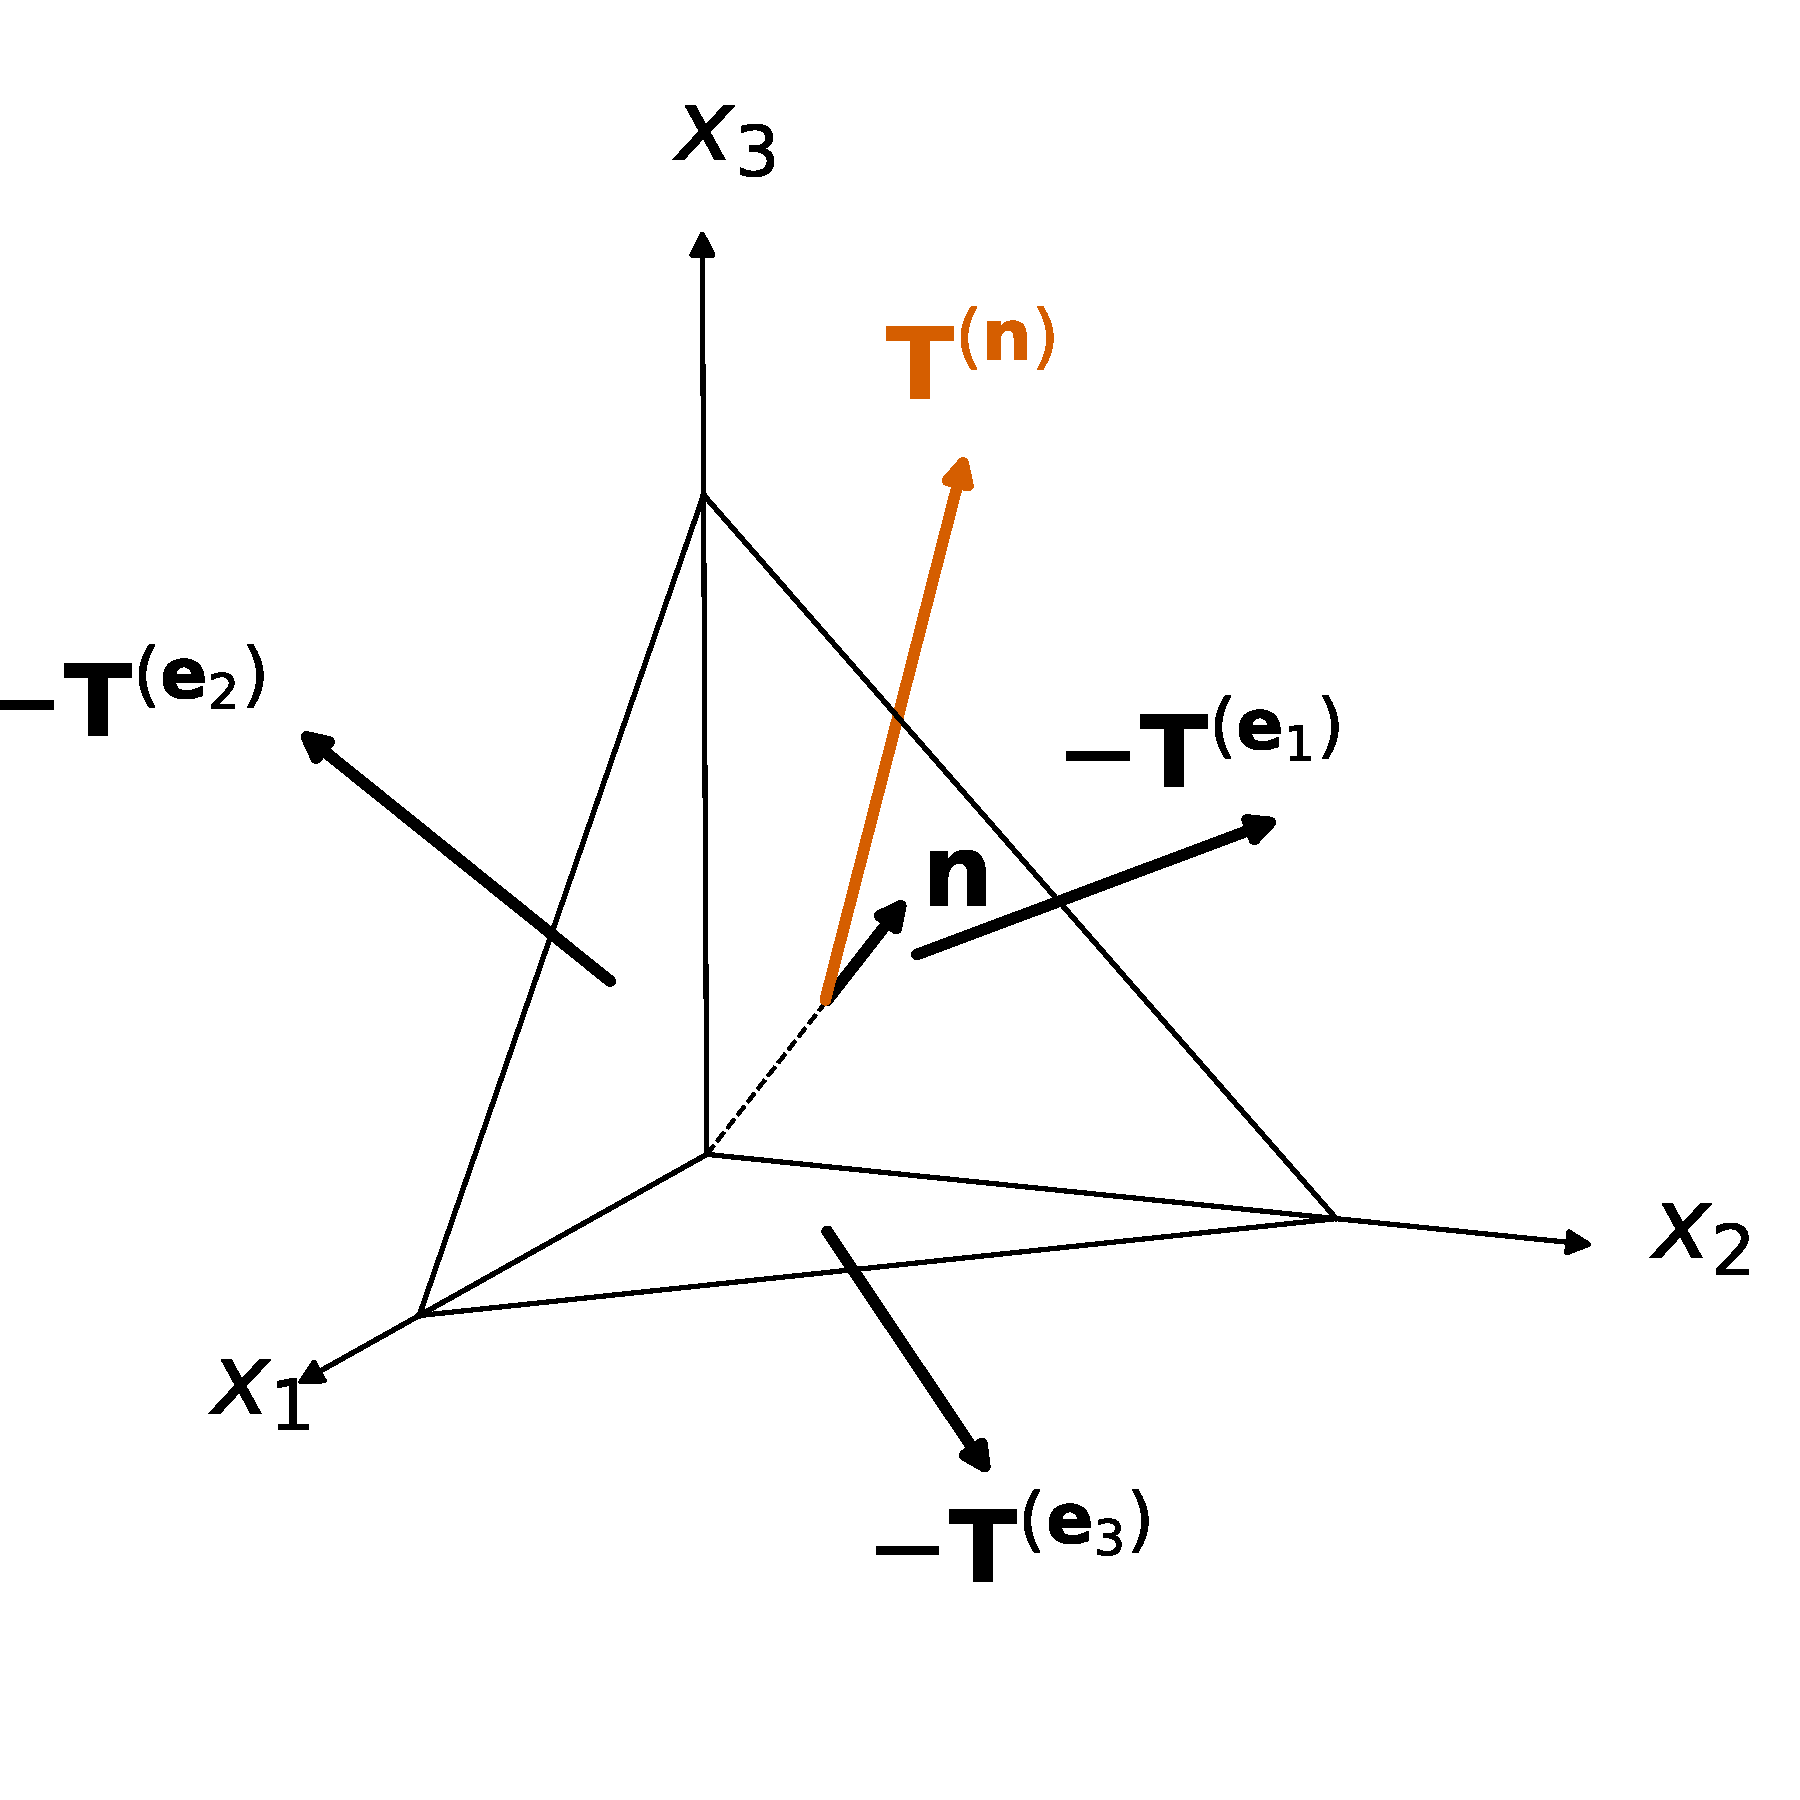
\includegraphics[width=0.5\linewidth]{chapters/2-Background/Figures/cauchy_tetrahedron.pdf}
    \caption[Force equilibrium on a Cauchy tetrahedron for the derivation of the traction vector.]{Cauchy tetrahedron used to derive the traction vector on an arbitrary plane from force equilibrium, relating stress components on coordinate planes to the stress acting on an inclined plane.}
    \label{fig:CauchyTetrahedron}
\end{figure}

This linear relation can be written in as
\begin{equation}
    \bm{s}(\bm{n}) = \bm{\sigma}\cdot\bm{n} \qquad (\textrm{or in components, } s_i = \sigma_{ij} n_j).
\end{equation}
This relation defines the Cauchy stress tensor $\bm{\sigma}$. As we defined the three faces of the tetrahedron to be aligned with the coordinate planes, the stress tensor in three dimentional cartesian corrdinates can be constructed as
\[
    \bm{\sigma} = 
    \begin{bmatrix}
    | & | & | \\
    \bm{s}^{(x)} & \bm{s}^{(y)} & \bm{s}^{(z)} \\
    | & | & |
    \end{bmatrix}
    = 
    \begin{bmatrix}
        \sigma_{xx} & \sigma_{xy} & \sigma_{xz} \\
        \sigma_{yx} & \sigma_{yy} & \sigma_{yz} \\
        \sigma_{zx} & \sigma_{zy} & \sigma_{zz}
    \end{bmatrix}.
\]

As with the strain tensor $\bm{\epsilon}$, the components of the stress tensor $\bm{\sigma}$ have a clear physical interpretation. The diagonal components correspond to normal stresses, acting perpendicular to a surface, while the off-diagonal components correspond to shear stresses, acting parallel to the surface. In the absence of body torques, local torque balance implies that the stress tensor is symmetric, i.e., $\sigma_{ij} = \sigma_{ji}$.
In Cartesian coordinates, it may therefore be written as
\[
    \bm{\sigma} =
    \begin{bmatrix}
        \sigma_{xx} & \sigma_{xy} & \sigma_{xz} \\
        \sigma_{xy} & \sigma_{yy} & \sigma_{yz} \\
        \sigma_{xz} & \sigma_{yz} & \sigma_{zz}
    \end{bmatrix}.
\]

For notational clarity, throughout the remainder of the thesis we distinguish between local and bulk measures of stress. In continuum descriptions, the bulk stress tensor $\bm{\Sigma}$ is defined as the spatial average of the local stress,
\begin{equation}
    \Sigma_{ij}=\frac{1}{V}\int_V \sigma_{ij}(\bm{r})\, dV,
\end{equation}
and may differ from the local stress in the presence of spatial heterogeneity, such as that arising from plastic deformation. Throughout the thesis, $\bm{\Sigma}$ denotes a bulk or system-averaged stress, while the precise definition used in each model is introduced where needed in the corresponding chapter. In \cref{sec:Fatigue}, it is defined explicitly in the construction of the elastoplastic model used in this chapter, while in \cref{sec:Ultradelayed,sec:DoubleNetworks} we use the virial stress tensor defined in \cref{sec:virialStress}.

\subsection{Linear Stress--Strain Relation}

To relate stress and strain, we require a constitutive relation. In the simplest case, the stress is a linear function of the strain (Hooke's law),
\[
    \sigma_{ij} = C_{ijkm}\epsilon_{km},
\]
where $C_{ijkm}$ is a fourth-rank tensor, often called the stiffness or elasticity tensor.

For an isotropic material, the stiffness tensor can be expressed in terms of two independent elastic moduli, $\mu$ and $\lambda$ (the Lam\'e parameters). The stress can therefore be written as
\[
    \sigma_{ij} = \lambda \epsilon_{kk} \delta_{ij} + 2\mu \epsilon_{ij}.
\]

For incompressible materials, the first term is replaced by a hydrostatic pressure $p$ that enforces the incompressibility constraint. The stress therefore reduces to
\begin{equation}
    \sigma_{ij} = -p\delta_{ij} + 2\mu\epsilon_{ij},
    \label{eq:incompressibleStress}
\end{equation}
which is the form used later where incompressibility is assumed.

\subsection{Plasticity} \label{sec:Plasticity}
The description of stress and strain introduced above implicitly assumes that the deformation of the material is fully reversible, such that the material returns to its original configuration upon unloading. However, many materials deviate from this behaviour once the applied stress exceeds a characteristic threshold. Beyond this point, the response is no longer purely elastic and irreversible deformation occurs. Here, yielding denotes the onset of this irreversible response, whether through plastic rearrangements, bond rupture, or other local irreversible events. Such processes introduce history dependence in the system's response and, in some cases, may progress to fracture.

In contrast to elastic deformation, in which all strain is recovered upon unloading and the material returns to its initial configuration, plasticity refers to the ability of a material to undergo such permanent deformation under applied loading. Consequently, upon unloading the original state is not recovered upon unloading but instead retains a memory of its deformation history in its new configuration \cite{lubliner2008plasticity,Simo2000-ComputationalInelasticity,Wu2004}. Microscopically these plastic deformation may correspond to particle rearrangements \cite{falk_dynamics_1998,maloney_amorphous_2006,tanguy_plastic_2006,gartner_nonlinear_2016}, dislocation \cite{shiba_plastic_2010, ispanovity_avalanches_2014,ben-zion_earthquake_1993}, or bond rupture \cite{tauber_stretchy_2022,ducrot_toughening_2014,Creton50th2017,vernereyStatisticalDamageMechanics2018,gong_why_2010} all of which reduce the total stored elastic energy. Rheologically, the sum of these microscopic deformations manifests as stress relaxation, yielding, and flow under sustained loading. 

\subsection*{Shear Banding} \label{sec:ShearBanding}

In the discussion so far, we have implicitly assumed that deformation is homogeneous across the material. However, this assumption can break down, and the strain may become spatially heterogeneous. An important example is shear banding, in which deformation localises into narrow bands that accommodate a large fraction of the total strain, while the surrounding material remains weakly deformed. Such shear bands are observed both experimentally \cite{manneville_recent_2008,divouxShearBandingComplex2016,berretTransientRheologyWormlike1997,berretNonlinearRheologyTelechelic2001,tapadiaBandingEntangledPolymer2006,goyonSpatialCooperativitySoft2008,besselingShearBandingFlowConcentration2010,divouxTransientShearBanding2010,rogersAgingYieldingShear2008} and theoretically  \cite{fielding_complex_2007,fielding_shear_2014,mfielding_shear_2009,fielding_triggers_2016,moorcroft_age-dependent_2011,carterShearBandingPolymeric,OlmstedShearBanding2008,doi_theory_1988} across a wide range of materials, including metallic glasses \cite{greer_shear_2013,SCHUH2007}, colloidal glasses \cite{aimeMicroscopicDynamicsFailure2018,besselingShearBandingFlowConcentration2010}, granular materials \cite{Shang2024,nessAbsorbingStateTransitionsGranular2020}, and polymeric materials \cite{carterShearBandingPolymeric,tapadiaBandingEntangledPolymer2006,moorcroft_shear_2014}.

\begin{figure}[b!]
    \centering
        \begin{subfigure}{0.45\textwidth}
        \centering
        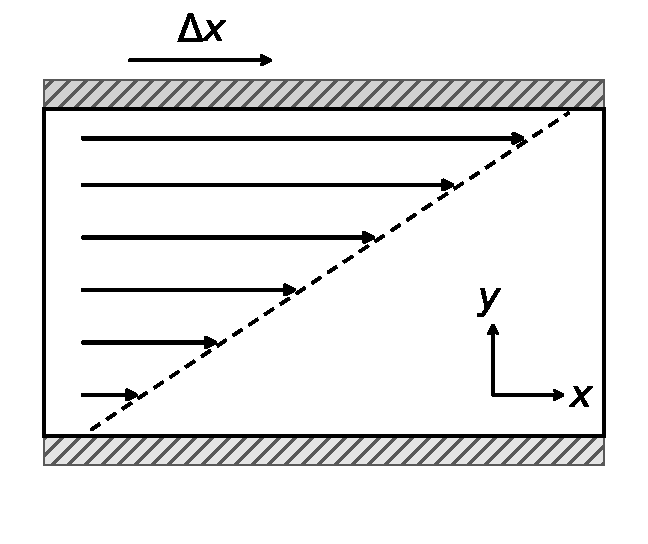
\includegraphics[width=\textwidth]{chapters/2-Background/Figures/ShearBanding_Homogeneous.pdf}
        \caption{Homogeneous deformation field}
        \label{fig:HomogeneousShear}
    \end{subfigure}
    \hfill
    \begin{subfigure}{0.45\textwidth}
        \centering
        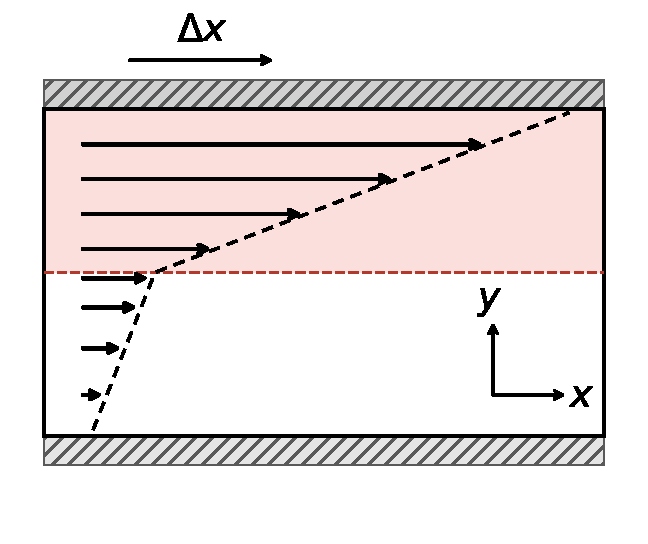
\includegraphics[width=\textwidth]{chapters/2-Background/Figures/ShearBanding_Localized.pdf}
        \caption{Shear banded deformation field}
        \label{fig:ShearBanded}
    \end{subfigure}
    \caption[Illustration of homogeneous shear and shear banding.]{Displacement profile examples for {\bf a)} a homogeneous displacement field and {\bf b)} a shear banded displacement field $u_x(y)$. Arrows indicate the direction and magnitude of the displacement. The cell is comprised of two parallel plates; the top plate is moved in the $x$ direction by a distance $\Delta x$, while the bottom plate is fixed. Spatial invariance in the $x$ and $z$ directions is assumed.
    }
    \label{fig:shearBandSketch}
\end{figure}

In simple shear, with flow along $x$ and gradient along $y$, this localisation corresponds to a spatially varying shear strain,
\begin{equation}
    \gamma(y) = \frac{\partial u_x}{\partial y},
\end{equation}
which becomes strongly localised within the band. A schematic illustration contrasting homogeneous deformation and shear banding is shown in \cref{fig:shearBandSketch}. Under a simple shear deformation, the displacement field is heterogeneous, as illustrated in \cref{fig:HomogeneousShear}. However, in the presence of shear banding, the displacement field becomes localised within a narrow region, as shown as the red region in \cref{fig:ShearBanded}, where the shear strain $\gamma(y)$ is large, while the surrounding material experiences only a relativly small deformation.

In many disordered solids, such as metallic glasses \cite{greer_shear_2013}, shear banding can be understood as the result of a mechanical instability of the homogeneous state. In particular, if the material exhibits strain softening, such that the stress decreases with increasing strain, $\partial_{\gamma}\sigma < 0$, then a uniformly deformed state becomes unstable \cite{barlow_ductile_2020}. Small spatial variations in strain are then amplified under continued loading, since regions that deform slightly more undergo local softening, resulting in a reduced stress required for further deformation and hence continued localisation. This positive feedback leads to the formation of a shear band, which is sustained under continued deformation.

Depending on the applied deformation protocol and material properties, these localised regions may either persist or evolve in time. Of particular interest are transient shear bands, which form during the early stages of deformation but subsequently decay, leading to a return to a more homogeneous state \cite{moorcroft_age-dependent_2011,barlow_ductile_2020,divouxTransientShearBanding2010,adams_transient_2011}. These bands typically arise from an initial instability of the homogeneous deformation field. However, as the material evolves, the conditions that drive this instability are no longer satisfied, and the system relaxes towards a more uniform state. In experimental systems, the perturbations that trigger this instability may arise from structural heterogeneity or thermal fluctuations.

Alternatively, in some cases, deformation becomes permanently concentrated within well-defined bands that accommodate most of the strain and act as precursors to macroscopic failure \cite{greer_shear_2013,hufnagel_deformation_2016,nicolas_deformation_2018,Falk2003,maloney_amorphous_2006,Shi2007,falk_deformation_2011,Barrat2011}. In such systems, once a dominant band has formed, subsequent deformation is largely confined to this region, leading to progressive weakening of the material along the band. This localised deformation is therefore self-reinforcing, ultimately leading either to catastrophic failure or to sustained, highly heterogeneous flow, as the surrounding material remains largely unloaded.

In general, shear banding reflects a competition between localising mechanisms, such as strain softening or yielding-induced weakening, and homogenising processes, including structural relaxation, and long-range elastic interactions \cite{fielding_shear_2014,divouxShearBandingComplex2016,martens_spontaneous_2012,moorcroft_criteria_2013,moorcroft_age-dependent_2011,nicolas_deformation_2018}. Whether deformation remains homogeneous, develops transient bands, or evolves towards persistent localisation is therefore determined by the balance of these effects and the imposed loading conditions \cite{fielding_shear_2014,divouxShearBandingComplex2016}. Understanding this competition is central to predicting failure and flow in disordered materials. In the following chapters, we will examine how these mechanisms emerge within the models considered here, and how they control the onset, evolution, and stability of strain localisation.

\section{Rheological protocol} \label{sec:Protocols}
There are many deformation protocols by which flow can be induced in a material, each probing different features of its mechanical response. In this work, we adopt strain-controlled deformation protocols, in which a prescribed bulk deformation is imposed at all times during the simulation, and the resulting stress response is measured. By contrast, in a stress-controlled protocol, a fixed (though potentially time-dependent) stress is imposed, and the material is allowed to deform accordingly \cite{macoskoRheologyPrinciplesMeasurements1994}. 

Within the linear elastic regime, stress- and strain-controlled protocols are equivalent because stress and strain are uniquely related by the elastic moduli. In the nonlinear regime, however, the two protocols can yield different responses. In stress-controlled experiments, the imposed stress can produce time-dependent deformation (creep) even below yielding, and, if sufficiently large, lead to sustained flow with effectively unbounded deformation. Such protocols are therefore well suited to probing both creep and the onset of yielding through the transition from arrested or weakly creeping states to continuous flow. By contrast, in strain-controlled experiments, the deformation history is prescribed and the stress is measured as the material response. These protocols are particularly well suited to resolving the evolution of stress through yielding, including post-yield stress redistribution, which is the focus of this thesis.

We will consider two forms of deformation in this thesis: simple shear is used in \Cref{sec:Fatigue,sec:Ultradelayed} and elongational stretching in \Cref{sec:DoubleNetworks}. In addition, each chapter conciders a different strain-controlled protocol, which are illustrated in \cref{fig:ShearProtocols}.

\begin{figure}[p]
    \centering
    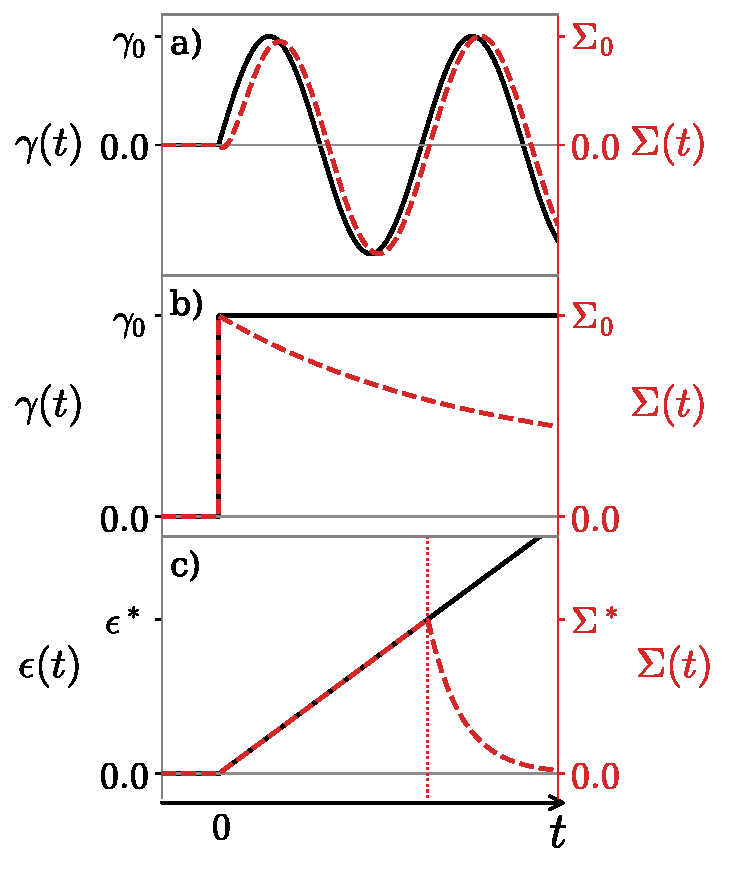
\includegraphics[width=0.8\linewidth]{chapters/2-Background/Figures/ShearProtocols.pdf}
    \caption[Diagram of deformation protocols]{Diagrams of the three deformation protocols studied in this thesis as functions of time. The imposed strain is shown by the solid black line, and a representative stress response is shown by the dashed red line. The strain is defined according to the relevant deformation mode in each chapter: $\gamma$ denotes the shear strain in \Cref{sec:Fatigue,sec:Ultradelayed}, and $\epsilon$ denotes the extensional strain in \Cref{sec:DoubleNetworks}. Although these protocols are illustrated for specific modes, they may be defined analogously for other types of deformation. The protocols are as follows: \newline
    {\bf a)} Large-amplitude oscillatory shear (LAOS), in which the strain varies periodically between $-\gamma_0$ and $\gamma_0$. \newline
    {\bf b)} Step strain, in which a strain of amplitude $\gamma_0$ is applied instantaneously at $t=0$ and then held constant. The material subsequently relaxes towards a new equilibrium state. \newline
    {\bf c)} Strain startup, in which deformation is imposed at a constant rate $\dot{\epsilon}$ for $t>0$. A brittle-like response is illustrated, where the stress initially increases with strain before dropping sharply at a critical strain $\epsilon^*$.
    }
    \label{fig:ShearProtocols}
\end{figure}

\subsection{Oscillatory Strain} \label{sec:lAOS}

Oscillatory shear is a widely used protocol for characterising the rheology of soft materials, with large-amplitude oscillatory shear (LAOS) being particularly well studied \cite{rouyerLargeAmplitudeOscillatory2008a,yoshimuraResponseElasticBingham1987a,viasnoffHowAreColloidal2003,carterShearBandingPolymeric,ewoldtLargeAmplitudeOscillatory2010,renouYieldingProcessesColloidal2010}. In a conventional experiment, the strain is prescribed as a sinusoidal function of time,
\[
    \gamma(t) = \gamma_0 \sin(\omega t),
\]
where $\gamma_0$ is the strain amplitude and $\omega$ sets the timescale over which the deformation is applied. For small amplitudes, $\gamma_0 \ll 1$, the response is linear as the material behaves elastically and can be expressed in terms of the storage and loss moduli, which quantify the elastic and viscous contributions to the stress. At larger amplitudes, the response becomes nonlinear, leading to waveform distortion and the appearance of higher harmonics in the stress signal, which provide a sensitive probe of yielding and dissipative processes within the material \cite{ewoldtLargeAmplitudeOscillatory2010}.

In addition to resolving the intra-cycle response, oscillatory shear provides access to the evolution of the material over successive cycles. In many amorphous systems, repeated driving leads either to the emergence of periodic, reversible responses in which the system returns to the same configuration each cycle, or to progressively evolving dynamics associated with irreversible rearrangements. The former corresponds to absorbing or limit-cycle states, while the latter reflects the latter underpins fatigue, in which plastic deformation accumulates over many cycles and can ultimately lead to yielding or failure \cite{liuFateShearoscillatedAmorphous2022,Leishangthem2017,Fiocco_memory_2014,Regev_onset_2013}. Oscillatory shear is therefore particularly well suited to probing the transition between reversible and irreversible behaviour in driven amorphous materials. 

In \cref{sec:Fatigue}, we consider the quasi-static limit of this protocol, in which the driving frequency is taken to be small compared to the intrinsic relaxation timescales of the material, $\omega \to 0$. In this limit, inertial and rate-dependent effects are negligible and the system evolves through a sequence of mechanically equilibrated states, even as plastic events occur. Numerically, this corresponds to cycling the strain between $-\gamma_0$ and $\gamma_0$ over successive cycles, stopping at strains where the material yields and evolving the system until it reaches a new equilibrium state before proceeding to the next step in the cycle. This protocol has become a common tool for probing the stability and memory of amorphous solids under repeated loading, as it emphasises the role of accumulated plastic activity while minimising rate-dependent effects \cite{liuFateShearoscillatedAmorphous2022,Leishangthem2017,Fiocco_memory_2014,Regev_onset_2013}.

\subsection{Step Strain} \label{sec:StepStrain}
In \Cref{sec:Ultradelayed} we focus on the step strain protocol. In this protocol, afer the sample is initialised, a strain of amplitude $\gamma_0$ is applied instantaneously at $t=0$ and is held constant for all subsequent times. The response is the charaterised by the evolution of the stress $\Sigma(t)$, which typically exhibits a rapid initial increase as the material is strained followed by a time-dependent decay as the sample relaxes towards a new equilibrium state. This relaxation reflects the progressive redistribution of internal stresses and provides a direct probe of the relaxation dynamics of the material

Mathermatically, the imposed strain may be modeled as 
\[
    \gamma(t) = \gamma_0 \Theta(t),
\]
where $\Theta(t)$ is the Heaviside function. Formally, this corresponds to a a Dirac delta function in the strain rate, $\dot{\gamma}(t) = \gamma_0 \delta(t)$. In Practice, however, an idealised step strain is physically impossible to achieve due to the finite inertia of rheological instruments. Nevertheless, a strain ramp applied on a timescale which is short compared with the intrinsic material relaxation time can be modelled effectively as an instantaneous step \cite{Fang_inhomogeneity_2011}.

The step strain protocol is particularly useful because it isolates the intrinsic relaxation processes of the material. In linear viscoelastic systems, the stress typically decays smoothly over time, reflecting a spectrum of relaxation times associated with the underlying microstructure \cite{macoskoRheologyPrinciplesMeasurements1994,larson_structure_1999}. In disordered and glassy materials, however, the relaxation may be highly nontrivial, exhibiting multiple timescales, slow decay, ageing, or delayed yielding following the initial deformation \cite{fielding_complex_2007,moorcroft_age-dependent_2011,lockwood_ultradelayed_2025}.

\subsection{Strain Startup} \label{sec:ShearStartup}

Another common protocol for characterising a material’s rheological response prior to steady flow or failure is strain startup, in which deformation is imposed continuously at a constant rate $\dot{\epsilon}$ for all times $t>0$ \cite{larson_structure_1999,tannerEngineeringRheology2000,barnes_introduction_1989}. This protocol probes how the material evolves from its initial undeformed state under sustained driving and provides a direct means of accessing the transient dynamics leading to yielding and steady flow. In particular, it allows one to resolve the progression from elastic loading, through yielding, to a flowing or plastically deforming state, and is widely used to identify elastic regimes, stress overshoots, and the onset of irreversible deformation \cite{divouxShearBandingComplex2016,moorcroft_age-dependent_2011}

For an ideal elastic solid, the stress increases linearly with strain, $\Sigma \propto \epsilon = \dot{\epsilon} t$, until a characteristic breaking or yield strain is reached, beyond which the material no longer responds elastically. By contrast, a Newtonian fluid exhibits a constant stress response, $\Sigma = \eta \dot{\epsilon}$, determined entirely by the imposed rate. Yield stress materials display behaviour intermediate between these limits: the stress initially increases approximately linearly with strain, reflecting an elastic regime, before approaching a steady-state value set by the flow curve. In many such materials, particularly in shear, the stress reaches a maximum (a stress overshoot) and subsequently relaxes towards a steady-state value $\Sigma(t \to \infty) = \Sigma_{\mathrm{steady}}(\dot{\epsilon})$ consistent with the underlying flow curve \cite{divouxShearBandingComplex2016,larson_structure_1999}. However, not all materials evolve towards steady flow under continued deformation. In some cases, the material is unable to sustain any applied load beyond a critical strain $\epsilon^*$, and instead undergoes fracture or catastrophic failure.

In \Cref{sec:DoubleNetworks}, we consider a quasi-static version of this protocol, in which the imposed deformation is applied sufficiently slowly that the system remains close to mechanical equilibrium at all times, corresponding to $\dot{\epsilon} \to 0$. In this limit, inertial and finite-rate effects are negligible, and the response can be interpreted as a sequence of mechanically equilibrated states, allowing the onset of plasticity and failure to be resolved in terms of the underlying structural evolution.

% \subsection{Experiments} \label{sec:Experements}

% In order to understand these nonlinear effects, which are often controlled by the dynamics of internal microstructure, experimental rheologists use a number of experimental techniques which often involve shearing a material between two plates.

\section{Force balance in the Stokes limit} \label{sec:Hydrodynamics}

The constitutive descriptions introduced above specify how local stress responds to deformation. Across this thesis, we also require a general framework for how stress relaxes and redistributes after local perturbations, including plastic rearrangements in mesoscopic models and bond-level damage in networks. In soft disordered materials, this redistribution is governed by incompressible hydrodynamics in the low-Reynolds-number limit. We therefore summarise the corresponding force-balance equations in a form used throughout this thesis.

% \subsection{Navier-Stokes}
% From conservation of mass and momentum, the Navier--Stokes equations for a generalised incompressible flow read
% \begin{subequations}
% \label{eq:NavierStokes}
% \begin{align}
%     \rho \left(\partial_t+(\bm{u} \cdot \nabla)\right)\bm{u} &= \nabla \cdot \bm{\sigma} \label{eq:incompressibleNavier1} \\
%     \nabla\cdot\bm{v} &= 0 \label{eq:incompressibleNavier2}
% \end{align}
% \end{subequations}

% where $\rho$ is the fluid's density, $\bm{v}$ the fluid's flow field, and $\bm{\sigma}$ is a tensor which characterises the total stress applied to the fluid. The total stress may be decomposed as $\bm{\sigma} = \bm{\tau} - p\bm{I}$, where $\bm{\tau}$ is the deviatoric stress tensor and $p$ is the hydrostatic pressure.

% The physics we wish to consider in this thesis is the slow flow of pasty materials where the internal viscous forces dominate over the inertial forces. We therefore consider the low-Reynolds-number limit of \cref{eq:incompressibleNavier1} as 
% \[
%     Re=\rho U L / \mu \to 0
% \]
% where $U$ and $L$ are characteristic displacements and length scales. In this limit, the inertial term on the left-hand side of \cref{eq:incompressibleNavier1} becomes negligible, and the equations reduce to
% \begin{subequations}
% \label{eq:StokesLimit}
% \begin{align}
%     \nabla \cdot (\bm{\tau} - p\bm{I}) &= 0 \\
%     \nabla \cdot \bm{u} &= 0.
% \end{align}
% \end{subequations}
% This result may also be obtained directly from the mechanical equilibrium condition in \cref{eq:incompressibleStress}, which requires the net force in the system to vanish:
% \[
% \nabla \cdot (\mu \bm{\epsilon}) = \nabla \cdot \bm{\sigma} = 0.
% \]

\subsection{Navier-Stokes}
From conservation of mass and momentum, the Navier--Stokes equations for a generalised incompressible flow read
\begin{subequations}
\label{eq:NavierStokes}
\begin{align}
    \rho \left(\partial_t+(\bm{v} \cdot \nabla)\right)\bm{v} &= \nabla \cdot \bm{\sigma} \label{eq:incompressibleNavier1} \\
    \nabla\cdot\bm{v} &= 0 \label{eq:incompressibleNavier2}
\end{align}
\end{subequations}
where $\rho$ is the fluid density, $\bm{v}$ the velocity field, and $\bm{\sigma}$ the total Cauchy stress tensor. The stress may be decomposed as
\begin{equation*}
    \bm{\sigma} = \bm{\tau} - p\bm{I},
\end{equation*}
where $\bm{\tau}$ is the deviatoric stress tensor and $p$ the hydrostatic pressure enforcing incompressibility.

The physics considered in this thesis concerns the slow deformation of soft disordered materials, in which viscous and elastic stresses dominate over inertia. We therefore consider the low-Reynolds-number limit of \cref{eq:incompressibleNavier1},
\[
    Re = \frac{\rho v L}{\mu} \to 0,
\]
where $v$ and $L$ are characteristic velocity and length scales. In this limit, inertial terms become negligible and the equations reduce to the Stokes (force-balance) equations
\begin{subequations}
\label{eq:StokesLimit}
\begin{align}
    \nabla \cdot (\bm{\tau} - p\bm{I}) &= 0, \\
    \nabla \cdot \bm{v} &= 0.
\end{align}
\end{subequations}

In what follows, we adopt a displacement-based formulation. Introducing a displacement field $\bm{u}(\bm{r},t)$ with $\bm{v}=\partial_t\bm{u}$, the quasi-static limit corresponds to determining $\bm{u}$ at each time from the mechanical equilibrium condition \cref{eq:StokesLimit}. This result may also be obtained directly from the requirement that the net force vanish,
\[
\nabla \cdot \bm{\sigma} = 0.
\]

To connect this framework to models with local irreversible rearrangements (notably the elastoplastic model in \cref{sec:Fatigue}), we introduce a plastic eigenstrain field following Ref.~\cite{picard_elastic_2004}. Here, the eigenstrain $\bm{\epsilon}^{\mathrm{pl}}$ denotes a locally imposed, irreversible strain representing only the deformation generated by the rearrangement events themselves, excluding any elastic strain induced in the surrounding material.Assuming a homogeneous, isotropic, linearly elastic medium, the total strain may be written as
\begin{subequations}    \label{eq:decompositionAndDeformation} \label{eq:EPStrain}
\begin{gather}
    \bm{\epsilon} = \bm{\epsilon}^{\mathrm{el}} + \bm{\epsilon}^{\mathrm{pl}}
    \label{eq:strainDecomp} \\
    \bm{\epsilon} =
    \frac{1}{2}\left(\nabla \bm{u} + (\nabla \bm{u})^{T}\right)
\end{gather}
\end{subequations}
where $\bm{u}(\bm{r})$ is the total displacement vector at a position $\bm{r}$. For a homogeneous, isotropic, linearly elastic and incompressible medium ($\nabla\cdot\bm{u}=0$), the deviatoric stress becomes
\begin{equation}
    \bm{\tau} = 2\mu \bm{\epsilon}^{\mathrm{el}} = 2\mu\bm{\epsilon} - 2\mu\bm{\epsilon}^{\mathrm{pl}}.
    \label{eq:elasticStress}
\end{equation}

% Now, considering a single localised plastic event induced by elastic loading, the strain field $\bm{\epsilon}$ can be decomposed into a superposition of $\bm{\epsilon}^{\mathrm{el}0}$, $\bm{\epsilon}^{\mathrm{el}1}$ and $\bm{\epsilon}^{\mathrm{pl}1}$ where the superscript $0$ denotes the contribution from the elastic loading and $1$ the contribution from the localised plastic event. The materials deformation field can also be decomposed in the same way into a pair of deformation fields $\bm{u}^0$ and $\bm{u}^1$, which are the material's elastic and plastic responses respectively, so that $\bm{u} = \bm{u}^0 + \bm{u}^1$. As the elastic contribution must obey \cref{eq:StokesLimit} and the incompressibility condition $\nabla \cdot \bm{u}^0 = 0$, the plastic deformation $\bm{u}^1$ resulting from the localised plastic event must satisfy, 
% \begin{subequations}
%     \label{eq:plasticStokes}
%     \begin{align}
%         \nabla \cdot \left( 2\mu \bm{\epsilon}^{\mathrm{el}1} - p^1 \bm{I} \right) &= 2\mu \nabla \cdot \bm{\epsilon}^{\mathrm{pl}1}, \label{eq:plasticStokes1}\\
%         \nabla \cdot \bm{u}^1 &= 0.
%     \end{align}
% \end{subequations}

% Under the assumption that the deformation is isotropic and incompressible ($\nabla \cdot \bm{u} = \bm{0}$) for any deformation at rest, we can express the left-hand side of \cref{eq:plasticStokes1} as 
% \[\nabla \cdot \left( 2\mu \bm{\epsilon}^{\mathrm{el}1} - p^1 \bm{I} \right) = -\nabla p^1 + \mu \nabla^2 \bm{u}^1.\]

\subsection{Oseen Tensor} \label{sec:Oseen}
The solution to \cref{eq:StokesLimit} is well known and has been studied in a wide range of systems.

For a local plastic eigenstrain, the displacement field in an unbounded medium obeys
\begin{subequations}
\label{eq:Stokes}
\begin{align}
- \nabla p(\bm{r}) + \mu \nabla^2 \bm{u}(\bm{r}) &= 2\mu \nabla \cdot \bm{\epsilon}^{\mathrm{pl}}(\bm{r}), \label{eq:Stokes1} \\
\nabla \cdot \bm{u} &= 0. \label{eq:Stokes2}
\end{align}
\end{subequations}
where $(\nabla \cdot \bm{\epsilon}^{\mathrm{pl}})_i = \partial_j \epsilon^{\mathrm{pl}}_{ij}$. The displacement field can then be expressed as a convolution of this eigenstrain source with the Green's function $\mathbb{O}_{ij}(\bm{r},\bm{r}^\prime)$,
\begin{equation}
    u_i(\bm{r}) = -2\mu \int \mathbb{O}_{ij}(\bm{r}-\bm{r}^\prime)\,\partial_l^\prime \epsilon_{jl}^{\mathrm{pl}}(\bm{r}^\prime)\, d\bm{r}^\prime.
\end{equation}
The tensor $\bm{\mathbb{O}}$ was first derived by Oseen in 1927 \cite{oseen_neuere_1927} and refined by Burgers in 1939 \cite{Burgers1939}. In the present context, it provides the projection kernel that maps the eigenstrain source onto an incompressible displacement field. This Green-function structure is closely related to Eshelby's treatment of an inclusion with a prescribed internal transformation strain \cite{eshelby_determination_1997}.

To keep the chapter focused on the main ideas, we give only the final solutions used later here and refer the reader to \Cref{app:OseenDerivation} for the full derivation. The Oseen tensor is obtained as
\begin{equation}
    \hat{\mathbb{O}}_{ij} = \frac{1}{\mu k^2}\left( \delta_{ij} - \frac{k_ik_j}{k^2} \right).
    \label{eq:Oseen}
\end{equation}
which yields the displacement field in Fourier space,
\begin{equation}
    \hat{u}_i = -2\mu \hat{\mathbb{O}}_{ij} i k_l \hat{\epsilon}_{jl}^{\mathrm{pl}}
    = -\frac{2i}{k^2}\left( \delta_{ij} - \frac{k_ik_j}{k^2} \right) k_l \hat{\epsilon}_{jl}^{\mathrm{pl}}.
    \label{eq:fourierDeformation}
\end{equation}
and the corresponding deformation gradients,
\begin{equation}
    ik_m\hat{u}_i
    = 2\mu k_m \hat{\mathbb{O}}_{ij} k_l \hat{\epsilon}_{jl}^{\mathrm{pl}}
    = \frac{2 k_m}{k^2}\left( \delta_{ij} - \frac{k_ik_j}{k^2} \right) k_l \hat{\epsilon}_{jl}^{\mathrm{pl}}.
    \label{eq:fourierDeformationGradient}
\end{equation}
Both \cref{eq:fourierDeformation,eq:fourierDeformationGradient} naturally describe the deformation and deformation gradient fields for a infinite system up to an arbitrary constant $\bm{u}_0$, due to the singularity at $\bm{k}=\bm{0}$. We will address this constant later.

\subsection{Eshelby Stress Propagator} \label{sec:EshelbyPropogator}

We now use the deformation gradients obtained above to construct the corresponding strain and stress fields. This provides one concrete application of the mechanical-equilibrium framework: the Eshelby stress propagator describing elastic redistribution after a localised plastic event.

From \cref{eq:EPStrain}, the resulting strain fields
\begin{equation}
        \epsilon_{ij} = \epsilon_{ij}^{\mathrm{el}} + \epsilon_{ij}^{\mathrm{pl}} \implies \epsilon^{\mathrm{el}}_{ij} = \frac{1}{2}\left( \partial_i u_j + \partial_j u_i \right) - \epsilon_{ij}^{\mathrm{pl}}
        \label{eq:eshelbyStrain}
\end{equation}
and stress fields
\begin{equation}
    \tau_{ij} = 2\mu \epsilon^{\mathrm{el}}_{ij}
    \label{eq:eshelbyStress}
\end{equation}
can then be expressed in terms of the deformation gradients found in \cref{eq:fourierDeformationGradient}. For simplicity, we consider a two-dimensional system and focus on the elastic stress redistribution associated with a local plastic shear event $\epsilon_{xy}^{\mathrm{pl}}$, characterised by the corresponding stress component $\tau_{xy}$. This choice is made for convenience, as the same analysis can be carried out for any component of the resulting stress and eigen strain components. While the explicit form of the response differs between components and in three dimensions, the underlying mathematical structure of the formalism remains unchanged and extends straightforwardly to more general cases.

In two dimensions, the Fourier representations of the displacement components $u_x$ and $u_y$ take the form,
\begin{subequations}
\begin{align}
    \hat{u}_x &= -2\mu\left(\hat{\mathbb{O}}_{xx}ik_y + \hat{\mathbb{O}}_{xy} ik_x \right)\hat{\epsilon}_{xy}^{\mathrm{pl}}, \label{eq:ux}\\
    \hat{u}_y &= -2\mu\left(\hat{\mathbb{O}}_{yx}ik_y + \hat{\mathbb{O}}_{yy} ik_x \right)\hat{\epsilon}_{xy}^{\mathrm{pl}}. \label{eq:uy}
\end{align}
\end{subequations}
Substituting $\hat{u}_x$ and $\hat{u}_y$ into \cref{eq:eshelbyStrain,eq:eshelbyStress} and resolving for $\hat{\tau}_{xy}$, we obtain
\begin{align*}
    \hat{\tau}_{xy} = 2\mu \hat{\epsilon}^{\mathrm{el}}_{xy} &= \mu\left( i k_x \hat{u}_y + i k_y \hat{u}_x \right) - 2\mu\hat{\epsilon}_{xy}^{\mathrm{pl}}\\
    & = 2\mu^2 \left( k_y^2 \hat{\mathbb{O}}_{xx} + k_x^2 \hat{\mathbb{O}}_{yy} + 2 k_x k_y\hat{\mathbb{O}}_{xy} - \frac{1}{\mu} \right)\hat{\epsilon}_{xy}^{\mathrm{pl}}
\end{align*}
where we use the symmetry of the Oseen tensor $\hat{\mathbb{O}}_{xy}=\hat{\mathbb{O}}_{yx}$.

By collecting terms, we obtain the shear stress propagator $\mathbb{G}_{xy}$, which describes the stress redistribution produced by a single plastic event in an infinite medium:
\begin{equation}
\tau_{xy}(\bm{r}) = \mu \int \mathbb{G}_{xy}(\bm{r}-\bm{r}') \epsilon_{xy}^{\mathrm{pl}}(\bm{r}') \, d\bm{r}',
\end{equation}
where the Fourier-space kernel is
\begin{equation}
\hat{\mathbb{G}}_{xy}(\bm{k}) = -4\frac{k_x^2 k_y^2}{k^4}.
\label{eq:StressPropogator}
\end{equation}
We illustrate in \cref{fig:Propogator} the stress redistribution resulting from a single plastic event with $\epsilon_{xy}^{\mathrm{pl}} = -1$ at the origin.

\begin{figure}
    \centering
    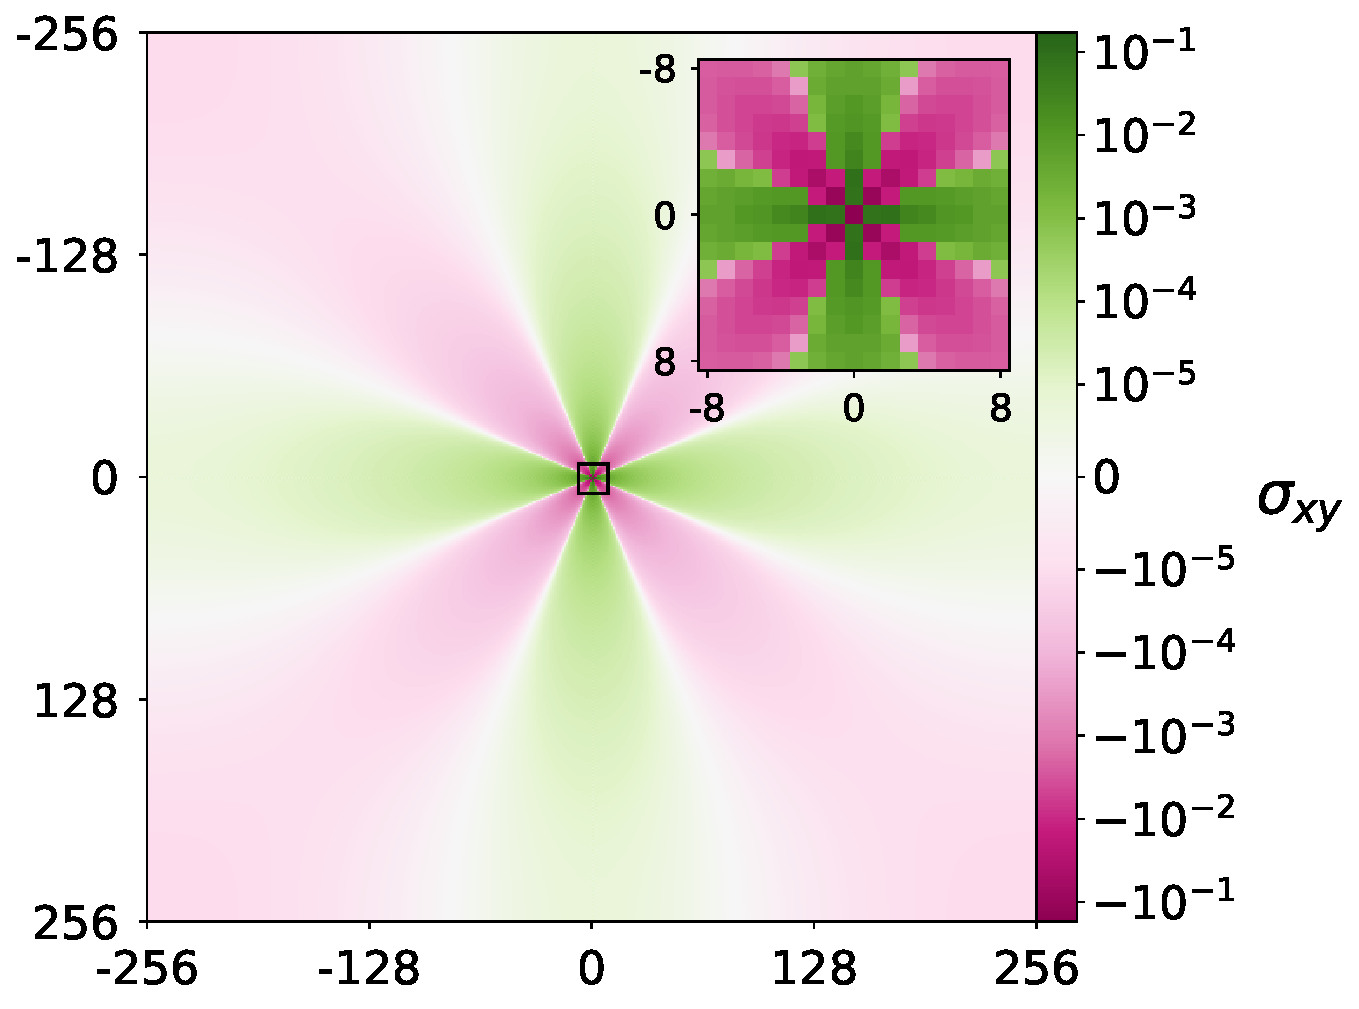
\includegraphics[width=0.75\linewidth]{chapters/2-Background/Figures/Prop_512_inset17.pdf}
    %\missingfigure{Plot of Propagator}
    \caption[Quadrupolar elastoplastic stress propagator]{Quadrupolar redistribution of shear stress $\tau_{xy}$ in two dimensions, after a single local plastic event in a system with $\mu=1$. The system is initialised with $\tau_{xy}=0$ everywhere; one central element is then yielded and set to $\tau_{xy}=-1$, after which mechanical equilibrium is enforced. The main panel shows the full $N_x\times N_y = 512\times512$ propagator, and the inset shows the central $17\times17$ region around the propagator.}
    \label{fig:Propogator}
\end{figure}

Equivalent expressions can be derived for the normal stress components $\tau_{xx}$ and $\tau_{yy}$, as well as for plastic events associated with normal stresses $\mu \epsilon_{xx}^{\mathrm{pl}}$ and $\mu \epsilon_{yy}^{\mathrm{pl}}$. Alternatively, the propagator may be generalised to three dimensions, for which
\begin{equation}
\hat{\mathbb{G}}_{xy}(\bm{k}) = -4 \frac{k_x^2 k_y^2}{k^4} - \frac{k_z^2}{k^2}.
\end{equation}
Expressing both the two- and three-dimensional kernels in the $xy$ plane, the real-space form asymptotically becomes
\begin{equation}
\mathbb{G}_{xy}(\bm{r}) \sim \frac{1}{r^{d}} \cos(4\theta),
\label{eq:eshelbyReal}
\end{equation}
consistent with the quadrupolar Eshelby field for an elliptical inclusion \cite{eshelby_determination_1997}. Consequently, in a system driven in simple shear, the stress perturbation generated by a local plastic event exhibits an eight-lobed structure: four lobes in which the shear stress increases and four in which it decreases (see \cref{fig:Propogator}).

The Eshelby stress propagator defined in \cref{eq:StressPropogator} is specified only up to an additive constant because of the singular mode at $\bm{k}=\bm{0}$. In practice, this constant is fixed by the boundary conditions. In a strain-controlled protocol, the total elastic strain is conserved. The zero mode is therefore chosen such that $\hat{\mathbb{G}}_{xy}(\bm{0}) = -1$, ensuring that the total stress relaxed by plastic events equals
\[
    \mu\int \epsilon_{xy}^{\mathrm{pl}}(\bm{r}^\prime) \, d\bm{r}^\prime.
\]

By contrast, under stress-controlled conditions, it is customary to set $\hat{\mathbb{G}}_{xy}(\bm{0}) = 0$. In this case, no net stress is removed from the system; instead, the stress released by plastic deformation is compensated by elastic loading of the surrounding material \cite{nicolas_deformation_2018,martens_spontaneous_2012,jocteur_protocol_2025,lin_scaling_2014}.

The form of the stress propagator given in \cref{eq:StressPropogator} is definded for an infinate mediu. However, it remains a good approximation for events sufficiently far from a solid wall or inclusion, due to its rapid $1/r^{D}$ decay. For a more rigorous treatment, the method of images may be used to simulate solid walls with a non-slip boundary condition to derive an equivalent Green function to the Oseen tensor (\cref{eq:Oseen}) \cite{blake_note_1971}, and also the stress propagator $\mathbb{G}_{xy}$ \cite{picard_elastic_2004}. However, for a two-dimensional system, it is often easier numerically to use an equivalent stream-function formalism as described in Ref.~\cite{acheson_elementary_1990}.

Although the explicit example above is written for plastic eigenstrains, the same Green-function viewpoint underpins stress relaxation more broadly throughout this thesis, including redistribution driven by bond-level rearrangements and failure in network models.

\section{Soft Networks} \label{sec:Networks}

The continuum framework outlined above provides a basic description of stress transmission and flow in soft materials and forms the foundation of the work considered in \cref{sec:Fatigue}. However, many of the systems of interest in this thesis derive their mechanical response from an underlying filamentous architecture that is not fully captured at this level. We therefore will adopt a mesoscale description in terms of soft networks, which retains the essential microscopic detail of how filaments are organised and connected, while remaining sufficiently coarse-grained to describe macroscopic behaviour. In such networks, the connectivity and arrangement of the constituent filaments play a central role in determining the emergent mechanics. The failure mechanisms of these networks are examined in detail in \cref{sec:Ultradelayed,sec:DoubleNetworks}.

\subsection{Types of Network} \label{sec:TypesOfNetworks}
With the term \quotes{soft networks}, we refer to materials made of interconnected filaments. While this shared structure suggests some network-level behaviour may be universal, key features remain material-specific. We therefore distinguish between generic precursors to failure and material-dependent mechanisms, to make clear where our models are expected to apply. Below, we briefly describe common classes of soft networks.

\paragraph{Elastomers:}
Composed of long, flexible polymer chains cross-linked into a network, elastomers are perhaps the best-known class of soft networks and are commonly found in thermosetting rubbers and plastics. Existing above the glass transition temperature $T_g$ of polymer networks, their mechanical behaviour is largely governed by entropic elasticity: deformation reduces the configurational entropy of polymer chains, generating a restoring force \cite{treloarElasticityRelatedProperties1973}. As a result, elastomers typically exhibit large reversible deformations until bond or cross-linker (i.e., molecules that connect distinct polymer chains together) failure occurs, with pronounced strain stiffening before failure \cite{kimMeasurementNonlinearMechanical2011}.

\paragraph{Hydrogels:}
As the name implies, hydrogels are a type of polymer gel Hydrogels are crosslinked polymer networks swollen with water, which can constitute up to around $90\%$ of the material volume \cite{gong_why_2010,tanaka_determination_2005,sun_highly_2012}. This high solvent content leads to a lower polymer density than in elastomers, resulting in materials that are typically softer and mechanically weaker. As a result of the low polymer volume fraction, interactions below the network scale are diminished, and the macroscopic properties become strongly dependent on the network structure. The presence of water also introduces additional physical phenomena, including swelling of the polymer chains and a coupling between network deformation and fluid flow, known as poroelasticity \cite{biotTheoryFiniteDeformations1972}. Owing to their high solvent content and mechanical compliance, hydrogels are widely explored for biomedical applications, particularly as artificial tendons, ligaments, and cartilage \cite{yasudaNovelDoubleNetworkHydrogel2009,yinSelfHealingHydrogelsSynthesis2023,hoHydrogelsPropertiesApplications2022}.

\paragraph{Fibre networks:}
Biological fibre networks are typically composed of semi-flexible filaments such as actin and collagen. These networks possess a characteristic length scale much larger than that of elastomers and hydrogels, with mesh sizes on the order of $1 \mu m$ to $10 \mu m$ \cite{mackintosh_elasticity_1995,Arevalo_Stress_Heterogeneities_2015}.
Much like hydrogels, these networks are highly porous, with a large fraction of their volume being occupied by solvent \cite{Jansen_Role_Collagen_2018}; however, due to their larger mesh size, they do not exhibit significant poroelastic effects \cite{Arevalo_Stress_Heterogeneities_2015}. The nature of crosslinking in such networks is also diverse, ranging from flexible linker proteins to branching and interwoven fibre bundles, leading to highly heterogeneous and mechanically complex interactions between filaments. Owing to their low fibre density, these materials typically exhibit a very small linear stiffness, making conventional extensional testing challenging in practice. As a result, their elastic and fracture behaviour is most commonly characterised under shear rather than through standard extensional protocols. Such fibre networks arise predominantly in biological contexts, where they provide structural support both within and outside cells \cite{burlaMechanicalResilienceActive2019}.

\paragraph{Colloidal networks:}
Colloidal networks consist of suspended particles that aggregate via short-range attractive interactions to form a space-spanning, percolated structure \cite{Mewis2011,nabizadeh_network_2024,Chen2020,zhang_correlated_2019}. These systems are typically out of equilibrium and evolve over time, exhibiting aging and restructuring as particle bonds rearrange \cite{viasnoffHowAreColloidal2003,renouYieldingProcessesColloidal2010,manley_gravitational_2005}. Mechanically, they behave as soft solids that can sustain stress at rest but yield and flow once interparticle bonds are disrupted, with properties strongly dependent on particle concentration and interaction strength \cite{Mewis2011}.

\paragraph{Macroscopic networks:}
Macroscopic network materials are systems in which the network structure can be directly observed with the naked eye. Common examples include textiles, fishing nets, and architected metamaterials. Such well-defined networks have also been used to study fracture and mechanical response \cite{driscollRoleRigidityControlling2016}. Their properties can vary widely depending on the material from which the network is made; however, the network architecture typically leads to behaviour that is softer and more extensible than that of the corresponding material in its bulk form. For example, a fishing net made of nylon fibres can stretch to several times its original length before breaking, even though nylon itself is relatively stiff and brittle.

To describe their mechanical response more precisely, it is necessary to consider the properties of the individual filaments that make up the network.

\subsection{Semi-Flexible Filaments} \label{sec:SemiFlexible}

Filaments can be broadly classified according to the ratio of their persistence length \(l_p\) to a relevant contour length \(l_c\), which in networks is typically taken as the mean distance between crosslinks. The persistence length quantifies filament stiffness and sets the length scale over which the filament orientation remains correlated. Intuitively, $l_p$ can be considered as the length scale at which thermal fluctuations of order $k_BT$ have a large enough effect to perturb the filament direction. More formally, it is defined through the decay of tangent--tangent correlations, $\langle \bm{t}(s) \cdot \bm{t} (0) \rangle = e^{-s/l_p}$, where $\bm{t}(s)$ is the tangent vector at a position $s$ along the filament backbone \cite{doi_theory_1988}. 

For short or stiff segments where $l_p \gg l_c$, the filaments act like a rigid rod with its mechanical response governed by enthalpic stretching of molecular bonds. For segments where persistence length is much smaller than the contour length $l_p \ll l_c$, thermal fluctuations are sufficient to induce significant bending, and the filament adopts a naturally coiled configuration. In this flexible region, the mechanical response is primarily entropic: small extensions reduce the number of accessible conformations, generating an effective restoring force. At larger extensions, the response again becomes governed by the enthalpic stretching of molecular bonds, as in the stiff case. 

Semi-flexible filaments, therefore, occupy an intermediate regime between these two limits, with a persistence length $l_p$ comparable to their contour length $l_c$. In this case, the filaments are stiff enough to avoid collapsing into a random coil but large enough that thermally induced bending remains relevant. 

The standard model for semi-flexible filaments is the extensible worm-like chain (EWLC), in which each filament is treated as a homogeneous cylindrical elastic rod of radius $r$ and Young's modulus $E$ \cite{doi_theory_1988}. The stretching rigidity of the rod is given by the product of its Young's modulus and cross-sectional area,
\[
    \mu = E \pi r^2,
\]
while the bending rigidity is determined by its Young's modulus and moment of inertia
\[
    \kappa = E I = E \pi r^4 / 4.
\]
The Hamiltonian of a single filament can therefore be written as the sum of two integrals, the stretching and bending contributions,
\begin{equation*}
    \mathcal{H} = \frac{\mu}{2} \int u(s)^2 \, ds + \frac{\kappa}{2} \int \left| \frac{\partial \vec{t}}{\partial s} \right|^2 \, ds
\end{equation*}
where \(u(s)\) denotes the local extensional strain and \(\bm{t}(s)\) the tangent vector at a position $s$ along the filament backbone. The second term penalises curvature and captures the bending energy of the filament, while torsional contributions are neglected.

\subsubsection*{Numerical Discretisation of Filaments}

In this thesis, we numerically discretise each filament into a series of segments, following Ref.~\cite{mackintosh_elasticity_1995}, The Hamiltonian of each filament can then be expressed as
\begin{equation}
    \mathcal{H} = \frac{\mu}{2} \sum_{ij} \frac{( l_{ij} - l_{ij,0} )^2}{l_{ij,0}} + \frac{\kappa}{2} \sum_{ijk} \frac{( \theta_{ijk} - \theta_{ijk,0} )^2}{l_{ijk,0}}.
    \label{eq:NetworkHamiltonian}
\end{equation}
The first sum runs over all pairs $ij$ along the filament backbone, while the second runs over all triplets $ijk$. Here $l_{ij}$ denotes the instantaneous segment length between nodes $i$ and $j$, and $\theta_{ijk}$ the instantaneous bond angle formed by nodes $i$, $j$, and $k$. Quantities with subscript $0$ denote their natural (not necessarily stress-free) values in the rest configuration. We further define $l_{ijk,0} = (l_{ij,0} + l_{jk,0})/2$. Multiple filaments can then be combined into a single network structure by connecting filaments at shared nodes, with the set of triplets $ijk$ updated accordingly. 

In this work, we restrict attention to central-force networks and therefore neglect bending rigidity, setting $\kappa = 0$. This approximation is justified in regimes where the mechanical response is dominated by the uniaxial stretching of filament segments rather than bending deformations. At the level of individual filaments, bending modes are generically much softer than stretching modes due to geometric scaling, with bending stiffness scaling as $EI \sim r^4$ and stretching stiffness as $EA \sim r^2$, such that slender filaments are comparatively easy to bend but resist extension. At the network level, in sufficiently connected or highly strained networks, these soft bending modes are progressively suppressed and the deformation becomes stretching-dominated, in which case the network elasticity is well captured by central-force interactions alone \cite{mackintosh_elasticity_1995,broedersz_criticality_2011,shivers_scaling_2019}. In this limit, the dominant contribution to the energy arises from changes in filament length, while angular distortions play a subleading role and may be neglected without qualitatively altering the mechanical response. Accordingly, we adopt a central-force description to isolate the role of network connectivity and axial elasticity in governing the behaviour studied in this thesis.

\subsection{Dynamics} \label{sec:NetworkDynamics}
To resolve the network dynamics, we assume overdamped motion in which elastic forces within the network are balanced at all times by a dissipative drag force arising from the surrounding solvent. The elastic force acting on node $i$, arising from filament stretching, is obtained from the Hamiltonian as
\begin{equation}
    \bm{F}_{n,i}=-\frac{\partial \mathcal{H}}{\partial \bm{r}_i}.
\end{equation}

This is balanced by a drag force from the solvent, $\bm{F}_{d,i}$, such that
\begin{equation}
    \bm{F}_{d,i} + \bm{F}_{n,i}=\bm{0}.
    \label{eq:ForceBalance}
\end{equation}

We neglect long-range hydrodynamic interactions in the drag term due to hydrodynamic screening arising from the network structure. In such networks, the fluid momentum is dissipated through friction with the network, leading to screening of hydrodynamic interactions beyond the mesh size \cite{shankar_theory_2002,visscher_dynamic_1994}. Instead, we consider a background Newtonian fluid with velocity field $\bm{v}_f(\bm{r}_i)$, which exerts a drag force on node $i$,
\begin{equation}
    \bm{F}_{d,i} = -\zeta\left(\dot{\bm{r}}_i - \bm{v}_f(\bm{r}_i)\right),
    \label{eq:Drag}
\end{equation}
where $\zeta$ is the drag coefficient. This form of drag is not Galilean invariant, as it depends on the absolute velocity of each node rather than relative velocities. However, it is widely used in the literature \cite{gittes_dynamic_1998,broedersz_modeling_2014,ikeda_unified_2012,puosi_time-dependent_2014,durian_foam_1995,salerno_avalanches_2012,liuDrivingRateDependence2016}, and yields results comparable to the more accurate form used in dissipative particle dynamics, in which dissipation is formulated in terms of pairwise relative velocities \cite{groot_dissipative_1997}. 

Deformations are imposed affinely at the level of the background flow, as in the affine solvent model \cite{durian_foam_1995,lerner_simulations_2013}, such that the fluid velocity field $\bm{v}_f$ follows the imposed macroscopic strain. The network nodes, however, are free to move non-affinely in response to the balance of elastic and drag forces.

\subsubsection{Integration Method} \label{sec:EulerHeun}
Rearranging \cref{eq:ForceBalance} and \cref{eq:Drag}, we obtain the equation of motion for the velocity of the $i$-th node,
\begin{equation*}
    \dot{\bm{r}}_i = \frac{1}{\zeta}\bm{F}_{n,i} + \bm{v}_f(\bm{r}_i).
\end{equation*}

To evolve the system numerically, we employ a splitting scheme in which the dynamics are decomposed into distinct contributions over each time step $\delta t$. Specifically, the displacement of each node is updated sequentially by (i) advection due to the background solvent velocity $\bm{v}_f$, and (ii) motion driven by elastic forces $\bm{F}_n$.

First, each node position, together with the system unit cell (see \cref{sec:Lees-Edwards} for implementation details), is advected affinely to account for the imposed flow field $\bm{v}_f$. The resulting advected position, $\bm{r}_i'$, is given by
\begin{equation*}
    \bm{r}_i' = \bm{r}_i(t) + \delta t \bm{v}_f(\bm{r}_i(t)).
\end{equation*}

In this thesis, deformations are either imposed instantaneously, as in \cref{sec:Ultradelayed}, or applied quasi-statically, as in \cref{sec:DoubleNetworks}. Under these conditions, the dynamics are effectively overdamped, and a first-order integration scheme is sufficient to capture the solvent drag and resulting node motion.

In the second substep, we employ an adaptive Euler--Heun method (also known as a Runge–Kutta 1(2) scheme) inspired by Ref.~\cite{sammullerAdaptiveBrownianDynamics2021}. This method uses an embedded Runge–Kutta pair, in which two solutions of different order are computed from the same intermediate evaluations to estimate the local discretisation error and adapt the time step $\delta t$. 

Starting from the advected position $\bm{r}^\prime_i$, we first compute the predictor estimate $\tilde{\bm{r}}_i$,
\begin{equation*}
    \tilde{\bm{r}}_i = \bm{r}^\prime_i + \frac{\delta t}{\zeta} \bm{F}_{n,i}(\bm{r}^\prime).
\end{equation*}

The forces are then re-evaluated at the predicted positions to obtain the corrected position at time $t+\delta t$:
\begin{equation*}
    \bm{r}_i(t + \delta t) = \bm{r}^\prime_i + \frac{\delta t}{2\zeta} \left[ \bm{F}_{n,i}( \bm{r}^\prime_i ) + \bm{F}_{n,i}(\tilde{\bm{r}_i}) \right].
\end{equation*}

The particle-wise error is defined as the difference between the first- and second-order updates,
\begin{equation*}
    E_i = \left\| \Delta\tilde{\bm{r}}_i - \Delta\bm{r}_i \right\| 
    = \frac{\delta t}{2\zeta}\left\| \bm{F}_{n,i}(\tilde{\bm{r}}_i) - \bm{F}_{n,i}(\bm{r}_i') \right\|_2,
\end{equation*}
where $\Delta\tilde{\bm{r}}_i = \tilde{\bm{r}}_i - \bm{r}_i'$ and $\Delta\bm{r}_i = \bm{r}_i(t+\delta t) - \bm{r}_i'$.

We introduce an error tolerance $\tau$, which constrains the maximum allowed absolute error. The global error estimate is then
\begin{equation*}
    \mathcal{E} = \left\| \frac{E_i}{\tau} \right\|_\infty,
\end{equation*}
where $\|\cdot\|_\infty$ denotes the maximum norm.

Following Ref.~\cite{sammullerAdaptiveBrownianDynamics2021}, we define the timestep scaling factor
\begin{equation*}
    q = \left( \frac{1}{2\mathcal{E}} \right)^2,
\end{equation*}
which is restricted to the interval $[0.001, 1.2]$. Two cases are then distinguished:
\begin{enumerate}
    \item $q \geq 1$: accept $\bm{r}_i(t+\delta t)$.
    \item $q < 1$: reject the step and restore the configuration to time $t$ before retrying with a smaller timestep.
\end{enumerate}

In both cases, the time step is updated via $\delta t \gets q \delta t$. We additionally impose a maximum time step $\delta t_{\max}$ to ensure adequate temporal resolution of fracture events.

\subsection{Rigidity} \label{sec:Rigidity}

One of the fundamental properties of soft network materials, absent from conventional continuum descriptions, is the origin of rigidity. In continuum elasticity, rigidity is assumed a priori through constitutive relations, and materials are taken to support stress under infinitesimal deformation. By contrast, in soft networks, mechanical stability emerges from a balance between constraints and degrees of freedom at the filament level. Consequently, a network's connectivity, topology, and filament mechanics collectively determine whether it can support stress. In the section that follows, we distinguish between two complementary origins of rigidity in soft networks: constraint-based rigidity, governed primarily by network connectivity, and strain-induced rigidity, which emerges under applied deformation through non-linear dynamics in the network.

We begin by considering rigidity arising from the number of constraints in the system. To do so, we examine idealised frameworks in which each connection has a fixed length $l_{ij,0}$ and can freely hinge at its nodes, with no bending penalty. This corresponds to the limit of \cref{eq:NetworkHamiltonian} with $\mu \to \infty$, enforcing $l_{ij} = l_{ij,0}$, and $\kappa = 0$.

Defining $\bm{r}_i(t)$ as the position of the $i$th node of the system, the network configuration is specified by the set of constraints
\[|\bm{r}_i(t) - \bm{r}_j(t)|^2 = l_{ij,0}^2\] 
imposed for all connected pairs $ij$. By differentiating with respect to $t$, this yields a set of compatibility conditions on the nodal velocities $\dot{\bm{r}}$,
\begin{equation} \label{eq:FrameworkRigidity}
    (\bm{\dot{r}}_i(t) - \bm{\dot{r}}_j(t))\cdot(\bm{r}_i(t) - \bm{r}_j(t))=0
\end{equation}
for every connected pair $ij$.

If there exists a non-trivial set of velocities $\dot{\bm{r}}_i$ satisfying \cref{eq:FrameworkRigidity}, the framework admits an infinitesimal deformation (a floppy mode), as at least one node can be moved freely, and the structure is not first-order rigid. Conversely, the framework is defined to be first-order rigid if the only solutions to \cref{eq:FrameworkRigidity} are the trivial rigid-body motions. In simple terms, the network is first-order rigid if the constraints allow for a single unique configuration (up to rigid-body translations and rotations).

This idea is most simply understood through a counting argument due to Maxwell \cite{maxwell_calculation_2011}, in which rigidity is determined by comparing the number of constraints to the number of degrees of freedom. For a $d$-dimensional system of $N$ nodes, there are $dN$ translational degrees of freedom, corresponding to the independent displacements of each node. However, not all of these contribute to internal deformation: $d$ degrees of freedom correspond to uniform translations of the entire system, and $d(d-1)/2$ correspond to rigid-body rotations, which leave all distances between nodes unchanged. Subtracting these trivial modes, the number of non-deforming degrees of freedom is $d(d+1)/2$, leaving $dN - d(d+1)/2$ non-trivial degrees of freedom. The total number of constraints $N_c$ needed for the system to be first-order rigid must therefore be at least equal to the number of non-trivial degrees of freedom
\[
    N_c \geq d N - d ( d+1 ) / 2.
\]
Assuming the network is homogeneous, we define the average connectivity as $z=2N_c/N$, where a bond between two nodes contributes one constraint. In the thermodynamic limit $N \to \infty$, this yields the condition $z \ge 2d$ for rigidity. The critical point $z_c = 2d$ is referred to as the isostatic point. More generally, networks are classified according to their connectivity relative to this point: sub-isostatic networks possess fewer constraints than degrees of freedom and admit floppy modes, isostatic networks are marginally rigid, and hyperstatic networks contain redundant constraints and can support states of self-stress \cite{LernerCoordination2024,Mao2018,ellenbroek_rigidity_2015,wyart_elasticity_2008}.

% This idea is more simply understood through the work of Maxwell \cite{maxwell_calculation_2011}, who initially pointed out that this definition of rigidity is directly related to the number of constraints in the system. For a $d$-dimensional system of $N$ nodes, the condition for the number of constraints $N_c$ for the system to be rigid is 
% \[
%     N_c \geq d N - d ( d+1 ) / 2.
% \]
% Assuming the network is homogenous, we can define an average connectivity of the network $z=2N_c/N=2N_B/N$, where $N_B$ is the number of bonds in the system. By letting $N\to\infty$, then for a homogenous network to be rigid, $z\geq 2d$. The critical point $z_c=2d$ is often referred to as the isostatic point. More generally, networks are classified according to their connectivity relative to the isostatic point: sub-isostatic networks possess fewer constraints than degrees of freedom and admit floppy modes, isostatic networks are marginally rigid, and hyperstatic (over-constrained) networks contain redundant constraints and can support states of self-stress \cite{LernerCoordination2024}.

This first-order rigidity criterion holds only when the network forms a single rigid cluster and the bond constraints are independent. In general, however, these conditions need not be satisfied, particularly in over-constrained systems. In such networks, states of self-stress can arise, defined as assignments of internal forces that satisfy force balance in the absence of external loading. The presence of these redundant constraints means that the number of independent constraints is smaller than the total number of bonds, and consequently the relationship between degrees of freedom and constraints cannot, in general, be inferred from simple counting arguments alone \cite{calladine_buckminster_1978}.

Often, this definition of first-order rigidity is overly restrictive and does not fully capture the behaviour of heterogeneous networks, for which the average connectivity $z$ alone is insufficient to determine rigidity. This limitation is particularly relevant for the disordered networks considered in later chapters.

As a simple example, consider attaching a single freely hanging node to an otherwise rigid network. This addition formally violates the strict definition of first-order rigidity, since the new node introduces a floppy mode. However, it does not alter the global load-bearing capacity of the original rigid cluster, which remains able to support stress. For such systems, it is necessary to consider not only the number of constraints but also their spatial organisation to determine global rigidity. In particular, sparsely connected networks below the isostatic point often consist of small rigid clusters embedded within floppy, under-constrained regions. In strongly heterogeneous networks, even systems with average connectivity exceeding the Maxwell threshold $z_c = 2d$ can reorganise such that global deformation occurs without requiring the extension of any bonds. Consequently, the ability of a network to sustain stress is governed by the existence of a system-spanning rigid cluster capable of supporting states of self-stress. For this reason, the onset of global rigidity is commonly described as a rigidity percolation transition \cite{zhang_correlated_2019}. This should be distinguished from geometrical percolation, which identifies the formation of a purely connected path between opposite boundaries of the network and does not, in general, imply mechanical rigidity \cite{kendall_percolation_2009,broadbent_percolation_1957}. In two dimensions, this problem has been well studied \cite{ellenbroek_rigidity_2015} through algorithms such as the pebble game \cite{jacobs_algorithm_1997, jacobs_generic_1995}. Extending these definitions to provide rigidity in dimensions higher than two dimensions has been proven to be computationally intractable using current methods \cite{abbott_generalizations_2008}.

While the definitions above provide a framework for characterising structural, or first-order, rigidity, they do not account for the fact that the networks considered here consist of deformable springs rather than fixed-length linkages. It is well known that under-constrained (sub-isostatic) spring networks can undergo a rigidity transition at coordination number less than $z_c=2d$ \cite{feng_percolation_1984, sharma_strain-controlled_2016, wyart_elasticity_2008, feng_nonlinear_2016, vermeulen_geometry_2017, rens_micromechanical_2018}. 

The simplest illustration of such a transition is a string fixed at both ends. When the separation between the fixed ends is smaller than the contour length of the string, the string carries no tension and admits a floppy mode, offering no resistance to transverse deformation. However, once the fixed points are separated sufficiently that the string comes under tension, the floppy mode is removed, and the string can resist transverse deflection, thereby appearing mechanically rigid \cite{biot_mechanics_1965}. Although the connectivity remains fixed at $z = 2$, rigidity emerges through the development of internal tension rather than changes in network topology. The disordered networks studied in this thesis also undergo this transition. We therefore define a critical shear strain $\gamma_c$ as the strain at which a sub-isostatic network first develops a finite shear modulus, marking the onset of strain-induced stiffening.

This transition is often referred to as second-order rigidity \cite{connelly_second-order_1996}, where non-structural changes can cause the system to act as if it is in a rigid configuration. Mathematically, second-order rigidity is obtained by differentiating \cref{eq:FrameworkRigidity} with respect to time, yielding
\begin{equation*}
(\bm{r}_i(t) - \bm{r}_j(t))\cdot(\bm{\ddot{r}}_i(t) - \bm{\ddot{r}}_j(t)) + (\bm{\dot{r}}_i(t) - \bm{\dot{r}}_j(t))\cdot(\bm{\dot{r}}_i(t) - \bm{\dot{r}}_j(t)) = 0,
\end{equation*}
where $\ddot{\bm{r}}_i(t)$ is the acceleration of a node $i$. This criterion allows rigidity to arise even when non-trivial solutions to \cref{eq:FrameworkRigidity} exist, through the stabilising effect of internal force balance in the material. It therefore represents a weaker notion of rigidity, but one that still permits the network to support states of self-stress. Such configurations are significantly more difficult to predict \cite{holmes-cerfon_almost-rigidity_2021}, as they emerge from nonlinear geometric and mechanical effects that have been extensively studied in the context of frameworks and tensegrities \cite{connelly_frameworks_2022,connelly_second-order_1996,calladine_first-order_1991}. Indeed, determining whether a general planar spring network is rigid is NP-hard \cite{abbott_generalizations_2008}, and consequently, no simple, universally applicable criterion exists for establishing rigidity.

For systems composed of semi-flexible filaments with extensible bonds, both first- and second-order rigidity provide useful proxies for mechanical stability \cite{van_hecke_jamming_2010}. However, these kinematic criteria do not fully capture the complexity of the energy landscape explored by such networks. A more recent and intuitive perspective is provided by energetic rigidity \cite{damavandi_energetic_2022}, which characterises rigidity in terms of the local structure of the elastic energy landscape. In this framework, a configuration is defined to be rigid if any infinitesimal deformation increases the elastic energy, such that the network resides at a local minimum of the energy.

This viewpoint has yielded important insights into the mechanics of spring networks, vertex models, and jammed packings of soft particles \cite{damavandi_energetic_2022-1}, particularly in the presence of pre-stress, i.e. internal stresses that exist in the absence of external loading. Nevertheless, even the energetic criterion does not provide a fully predictive framework for determining rigidity in highly disordered networks.

\subsection{Fracture in networks}\label{sec:Fracture}
In \cref{sec:Plasticity}, the idea of plasticity and yielding in elastoplastic materials is discussed and is directly used in \cref{sec:Fatigue}. Throughout this thesis, yielding and fracture are treated as related but distinct mechanisms of irreversible failure. Yielding refers to the onset of irreversible deformation and loss of purely elastic response, whereas fracture additionally implies material separation or a substantial loss of structural connectivity and load-bearing capacity. In network materials, this distinction is particularly important because macroscopic failure typically emerges from the progressive scission of individual connections within a highly heterogeneous structure.

Generally, material failure is a complex problem, stemming from the large separation in length scales between the failure event (e.g. the rupture of a single bond) and the global failure of the material through the evolution of macroscopic cracks. At the microscopic level, fracture begins with the scission of individual connections between nodes that collectively grow into macroscopic failures \cite{Creton50th2017,ju_role_nodate,sanner_less_2025,higuchi_fracture_2018,bonnDelayedFractureInhomogeneous1998,teece_gels_2014}. However, there is generally no one-to-one mapping between the failure of a single bond and the resulting macroscopic fracture. Moreover, the range of time scales involved is also large: damage may accumulate slowly as the material is deformed, whereas macroscopic cracks can propagate rapidly across the system.

This challenge is further compounded by the inherent disorder present in real-world soft networks \cite{broedersz_modeling_2014,broedersz_criticality_2011,feng_nonlinear_2016}. Unlike ordered materials such as crystalline solids, which possess an inherent repeating unit cell and well-defined defect states that act as nucleation sites for fracture, disordered networks lack any obvious structural signature by which such critical defects can be identified. Furthermore, this inherent disorder and the large non-affine rearrangements which occur in the networks often lead to heterogeneity in the stress at the level of individual filaments (i.e. the load is not distributed evenly across the network) \cite{Liang2016,tauber_microscopic_2020,tauber_sharing_2021,broedersz_modeling_2014,storm_nonlinear_2005,bouzidNetworkTopologySoft2018}. Here networks redistribute stress through non-affine rearrangements, often delaying catastrophic failure \cite{shivers_scaling_2019,tauber_sharing_2021,ducrot_structure_2015, tominaga_molecular_2007}. Consequently, predicting when and where any individual bond may fail is challenging.

Experimentally, it has been shown that soft network materials, including elastomers, hydrogels, and fibre networks, can undergo very large deformations before visible macroscopic damage occurs \cite{gong_why_2010,Kim2021,ducrot_toughening_2014,Creton50th2017,aimeMicroscopicDynamicsFailure2018,storm_nonlinear_2005}. Experimental methods such as small-angle neutron scattering \cite{ducrot_structure_2015,tominaga_molecular_2007}, birefringence imaging \cite{gong_double-network_2003,zheng_how_2021}, and light scattering \cite{porr_probing_2025} have helped to reveal how stress is distributed across the network. 

Recent work on mesoscopic computational models, which provide a balance between structural details and computational cost, has characterised this stress distribution \cite{shivers_normal_2019,shivers_scaling_2019,LernerCoordination2024,storm_nonlinear_2005} as well as how fracture evolves \cite{tauber_microscopic_2020,tauber_sharing_2021,tauber_role_2020,dussi_athermal_2020}. In these models it is common to assign a local rupture threshold to each bond. For central-force network models, this is typically implemented by rupturing bonds whose strain exceeds a critical threshold $\lambda$ \cite{tauber_role_2020,dussi_athermal_2020}. This scale, therefore, plays a central role in determining the system dynamics \cite{tauber_microscopic_2020}. 

At higher breakage thresholds $\lambda$, bonds rupture only at higher extensions, typically beyond the critical strain $\gamma_c$, defined as the strain at which a subisostatic network first develops a finite shear modulus and begins to stiffen. At these large deformations, the stress appears to concentrate along paths within the network, often referred to as force chains, which become more apparent at higher strains \cite{ruiz-franco_force_2022,Heussinger2007}. Here second order rigidity controls the overall fracture response. Consequently, fracture is less sensitive to the proximity of the rigidity transition and instead reflects the heterogeneous load-bearing backbones that emerges at large strain \cite{Sarkar2022}.

In contrast to the low-$\lambda$ limit, where bond rupture occurs closer to $\gamma_c$ and the evolving force-chain network \cite{Sarkar2022} directly controls damage accumulation, the response at higher $\lambda$ is less strongly governed by these structures. Moreover, because stress is already highly localised along the evolving force chains, increasing system size or connectivity can promote a crossover towards more abrupt, crack-like failure, even in nominally sub-isostatic networks \cite{zhang_fiber_2017,driscollRoleRigidityControlling2016,dussi_athermal_2020,tauber_stretchy_2022}.

In \cref{sec:Ultradelayed,sec:DoubleNetworks} we consider the failure of soft network materials in two different situations. In \cref{sec:Ultradelayed}, we consider delayed timescales that can be associated with the thermal failure bonds \cite{tauber_role_2020,Bullerjahn2014,arruda_three-dimensional_1993,james_theory_1943,Skrzeszewska2010}. Here we explore the brittle to ductile transition seen extensively in networks under both increasing temperature and imposed shear deformation \cite{dussi_athermal_2020,ahmedBrittleDuctileTransition2014,ducrot_toughening_2014,tauber_role_2020}, characterising a material's response in both the high and low failure threshold regimes. In \cref{sec:DoubleNetworks} the failure of bonds in networks composed of multiple components is considered. Here, we resolve how load sharing and stress redistribution between interpenetrating networks modify damage accumulation and can dramatically enhance toughness compared to single-network systems.

\subsection{Disordered Network Models} \label{sec:NetworkStructure}
Throughout the literature, a wide range of network geometries has been considered. The simplest are affine isotropic models, which approximate the network response by considering a single filament subjected to an imposed deformation and averaging over all initial filament orientations \cite{mackintosh_elasticity_1995, storm_nonlinear_2005}. While such models provide a useful baseline in the limits of high connectivity $z$ or large bending stiffness $\kappa$, they fail to capture key physics arising from non-affine rearrangements and orientational disorder in real-world networks. To incorporate these effects, it is necessary to explicitly specify a network topology that describes how bonds connect the nodes of the network. 

In this work, we consider two classes of networks: those derived from lattice structures and those constructed from the packing of bidispersed soft particles. These topologies are idealised and are not intended to represent a specific experimental system directly, but rather to provide controlled model networks that capture generic features of disordered filamentous materials.

\subsubsection{Lattice-based networks} \label{sec:LatticeBasedNetworks}

Lattice-based networks are among the simplest network topologies commonly used to study mechanical properties \cite{jacobs_generic_1995,feng_percolation_1984,shivers_scaling_2019,sharma_strain-controlled_2016}. Frequently studied examples include two-dimensional square \cite{mao_soft_2010}, triangular \cite{broedersz_criticality_2011,feng_percolation_1984}, and honeycomb \cite{rens_nonlinear_2016} lattices. Owing to their straightforward construction relative to more disordered network types, and their numerical robustness arising from the uniform lattice spacing $l_0$, these networks provide a convenient and well-controlled framework for analysing the mechanical response of fibre networks.

Such networks are constructed by placing nodes on a regular grid defined by a set of lattice vectors and subsequently connecting these nodes according to a prescribed set of rules. For example, in a two-dimensional square lattice, the node positions are generated by the lattice vectors $(1,0)$ and $(0,1)$, with nearest-neighbour nodes connected along the horizontal and vertical directions, subject to the chosen boundary conditions. Other simple lattices, such as the triangular lattice, can be generated analogously, while more complex lattices may be derived from these fundamental cases. For instance, a hexagonal lattice can be obtained from a triangular lattice by imposing the additional constraint that each node has connectivity $z = 3$. Owing to their regular structure, such lattices exhibit highly predictable behaviour, characterised by discrete values of connectivity and bond length.

\begin{figure}[t]
    \centering
    % \missingfigure[]{Lattice based network structure}
    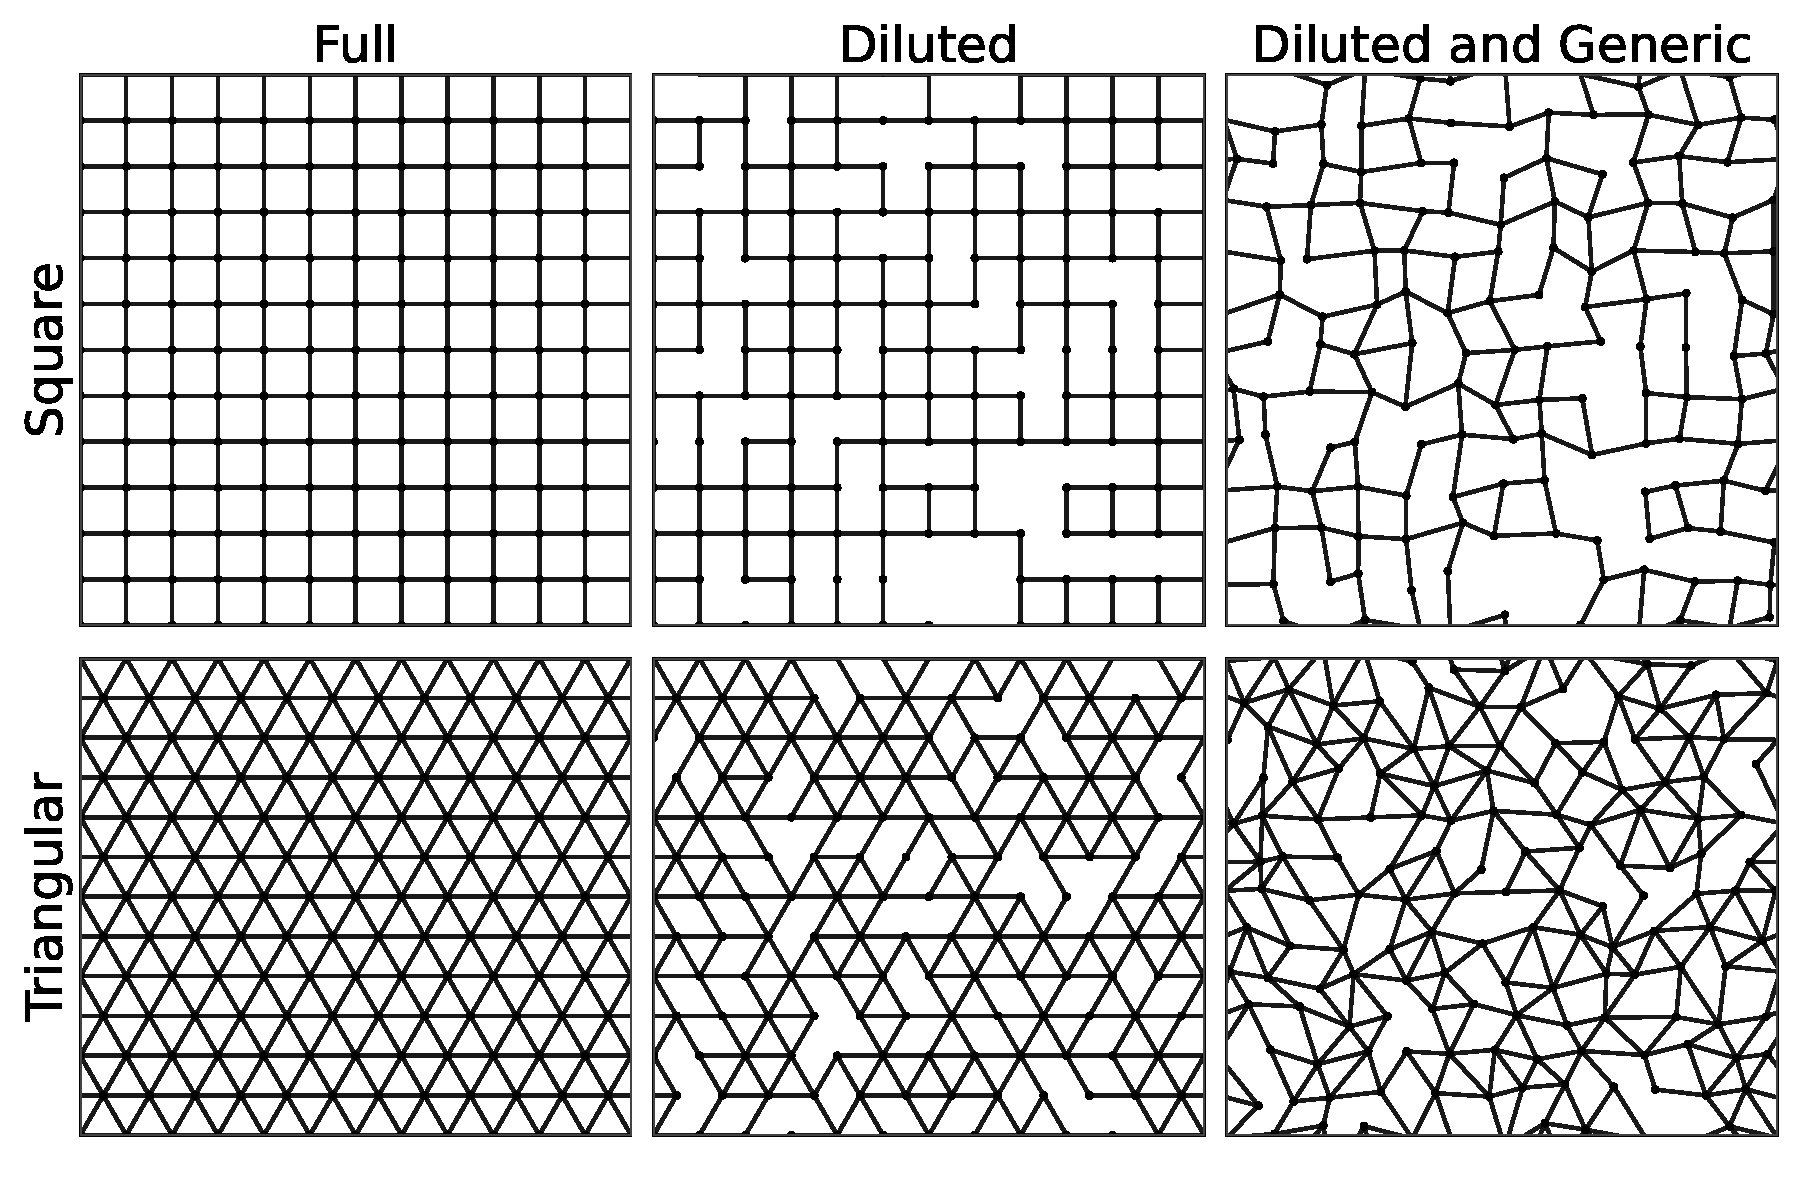
\includegraphics[width=0.95\linewidth]{chapters/2-Background/Figures/lattice_full_diluted_generic.pdf}
    \caption[Periodic lattices: full, diluted, and generic diluted networks.]{
    Examples of periodic lattice structures. We begin with regular lattices (\textbf{left column}), from which disordered diluted networks are generated (\textbf{centre column}) by randomly retaining bonds with probability $p=0.2$. Additional disorder is then introduced (\textbf{right column}) by displacing each node from its lattice position by a random distance $d \in [0,\delta_{\max}/2]$ in a random direction, yielding a generic diluted network. Here, $\delta_{\max}=0.6$ is expressed in units of the lattice spacing (i.e. the initial bond length). Dangling ends and dangling clusters are removed in all diluted networks shown (as described in \cref{sec:PrunningNetwork}).
    }
    \label{fig:LatticeNetworks}
\end{figure}

While trivial to construct, such lattices lack the structural disorder typical of disordered networks, which exhibit no long-range order. This predictability is undesirable when modelling disordered networks, where the goal is to represent amorphous materials lacking long-range structure. Disorder is therefore introduced into these networks through two complementary approaches. First, a common method is bond dilution via the random removal of lattice bonds. In practice, each bond is retained with probability $p$ (and removed with probability $1-p$), where $p$ sets the desired bond occupation fraction \cite{broedersz_criticality_2011,head_distinct_2003}. This procedure is widely used when studying the role of geometric percolation in such models \cite{broedersz_criticality_2011,feng_percolation_1984,das_redundancy_2012}.

Although random bond removal may appear to introduce only limited structural disorder, it fundamentally alters the rigidity of the network (see \cref{sec:Rigidity}). In particular, the system exhibits a rigidity percolation transition at a critical bond occupation probability $p_c$, at which isolated clusters coalesce into a single system-spanning cluster \cite{jacobs_generic_1995,zhang_correlated_2019}. A related transition occurs at the isostatic point, where the network loses (or gains) first-order rigidity.

A further advantage of bond dilution in lattice-based networks is the disruption of long, system-spanning force chains \cite{ruiz-franco_force_2022} that arise from the perfect alignment of bonds in the underlying lattice geometry. Networks that do not undergo such pruning typically exhibit low-strain softening of the shear modulus $K$ \cite{licup_nonlinear_2016}, associated with the buckling of these extended fibres.

The effects of these system-spanning force chains can be mitigated by a second form of disorder commonly employed in lattice networks, in which the nodal positions are randomly perturbed and the corresponding bond rest lengths and angles are redefined \cite{jacobs_generic_1995,krushynska_multi-frequency_2025,sheinman_nonlinear_2012,head_predicting_2025}. Networks incorporating this positional disorder are commonly referred to as generic networks \cite{jacobs_generic_1995}. The magnitude of these perturbations is typically constrained to be less than half the minimum lattice spacing, $\delta_{\min}/2$, to prevent node overlap \cite{shivers_normal_2019}. We explore the physics of square lattice based networks in \cref{sec:SquareAppendix} in the context of composite network materials comprising of two interconnected networks. 

\subsubsection{Packing-Derived Networks} \label{sec:PackingBasedNetworks}

Packing-derived networks are computationally constructed from simulated packings of soft particles and are widely used as model disordered networks \cite{rens_rigidity_2019,wyart_elasticity_2008,lerner_unified_2012,shivers_normal_2019,shivers_scaling_2019,shivers_phase_2022}. In practice, these networks are generated numerically by minimising the total energy of a bidisperse ensemble of soft disks at densities above the jamming transition $\phi_J$ \cite{Hernjamming2003,BoyerJamming2011,ikeda_unified_2012}, after which the contact network of overlapping particles is extracted and used to define the network connectivity. This procedure provides an idealised disordered topology and does not correspond to a specific experimental realisation, but instead serves as a controlled model for studying generic features of fibre and elastic networks.

Each disk is initially placed at a random position within a square periodic domain of size $L_x=L_y=\sqrt{N}$, with radii drawn from a bidisperse distribution with values $R_0$ and $fR_0$ in equal proportion. The bidispersity parameter $f$ is chosen to suppress crystallisation and inhibit the formation of long-range positional order; a commonly adopted value, and the one used throughout this thesis, is $f=1.4$. Such bidisperse mixtures are well known to produce amorphous packings with minimal macroscopic ordering \cite{van_hecke_jamming_2010, chacko_slow_2019, desmond_random_2009, koezeMappingJammingTransition2016}. 

The base radius $R_0$ is then rescaled so that the total particle area matches the prescribed packing fraction $\phi$ within the simulation box. While several forms of soft-disk interaction potentials have been proposed in the literature, we adopt the form used in Ref.~\cite{chacko_slow_2019}. In this model, overlapping disks interact via a purely repulsive pair potential given by
\begin{equation}
    U_{ij} \left(r_{ij}\right)
    = R_0^3\left(1-\frac{r_{ij}}{D_{ij}}\right)^2
    \Theta(D_{ij}-r_{ij}),
\end{equation}
where $r_{ij}$ is the centre-to-centre distance between disk $i$ and $j$, and $D_{ij}=R_i+R_j$ is the sum of their radii. The Heaviside function $\Theta(x)$ ensures that the interaction is non-zero only when particles overlap ($r_{ij}<D_{ij}$), and vanishes otherwise. 

Starting from this random initial condition, the system is relaxed via energy minimisation of the soft repulsive interactions until a mechanically stable packing is obtained. In Ref.~\cite{chacko_slow_2019}, this minimisation is performed by integrating an overdamped equation of motion equivalent to that presented in \cref{sec:NetworkDynamics}.

In the present work, however, our primary interest lies in the network structure obtained from the final minimised configuration rather than on the relaxation dynamics. We therefore generate packings using the Fast Inertial Relaxation Engine (F.I.R.E.) algorithm \cite{bitzek_structural_2006, guenole_assessment_2020}, which converges to local energy minima more efficiently. While this approach accelerates the energy minimisation, it does not capture physically accurate relaxation dynamics.

\begin{figure}
\centering
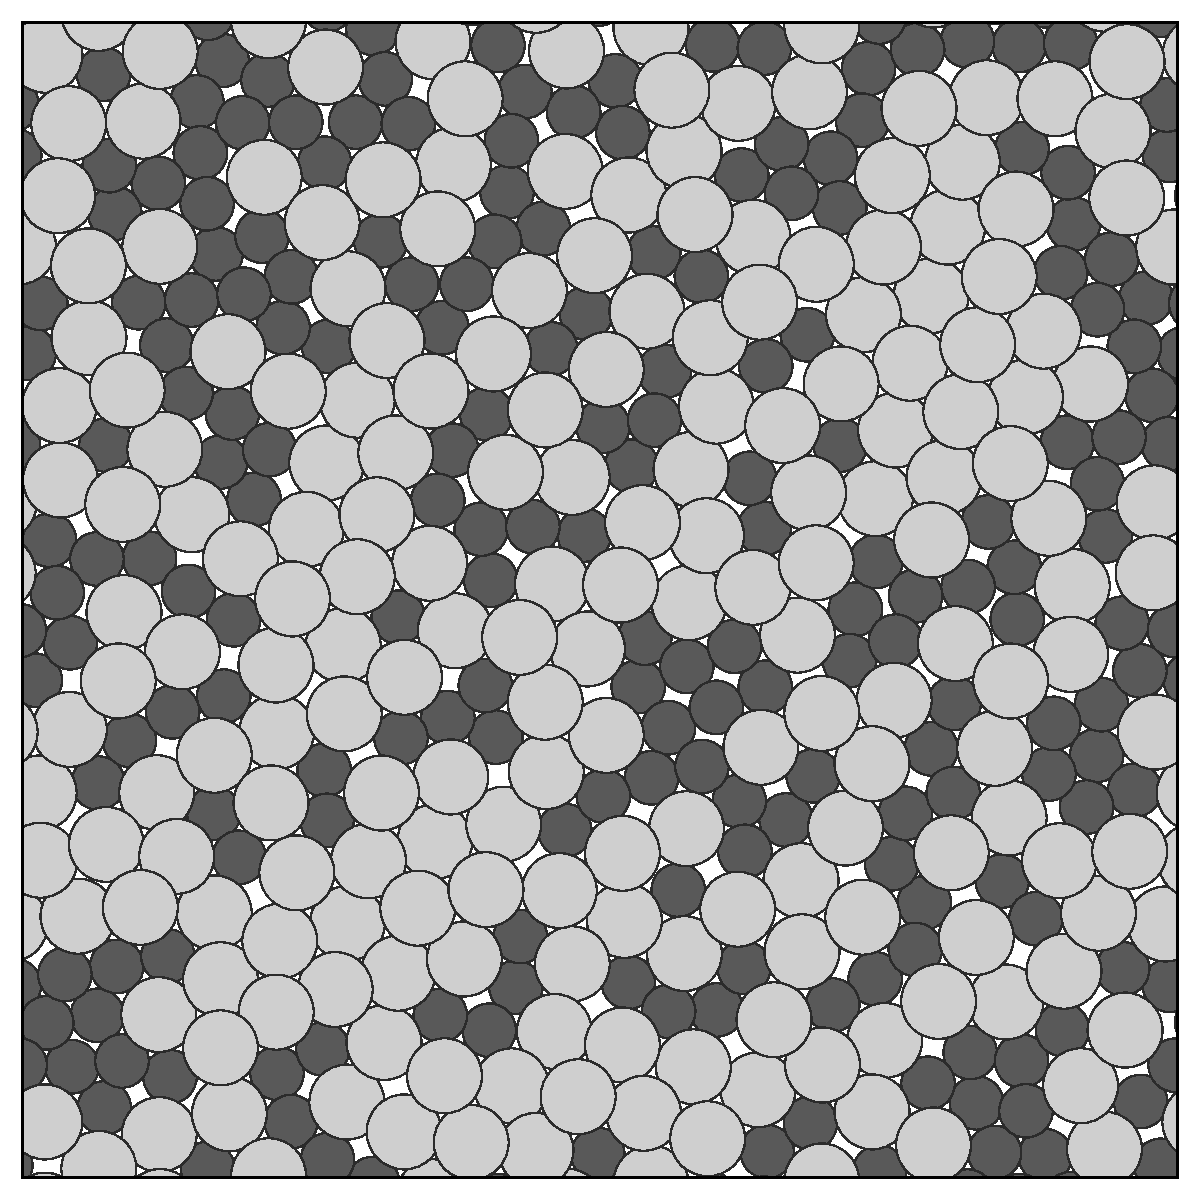
\includegraphics[width=.32\textwidth]{chapters/2-Background/Figures/particles.pdf}\hfill
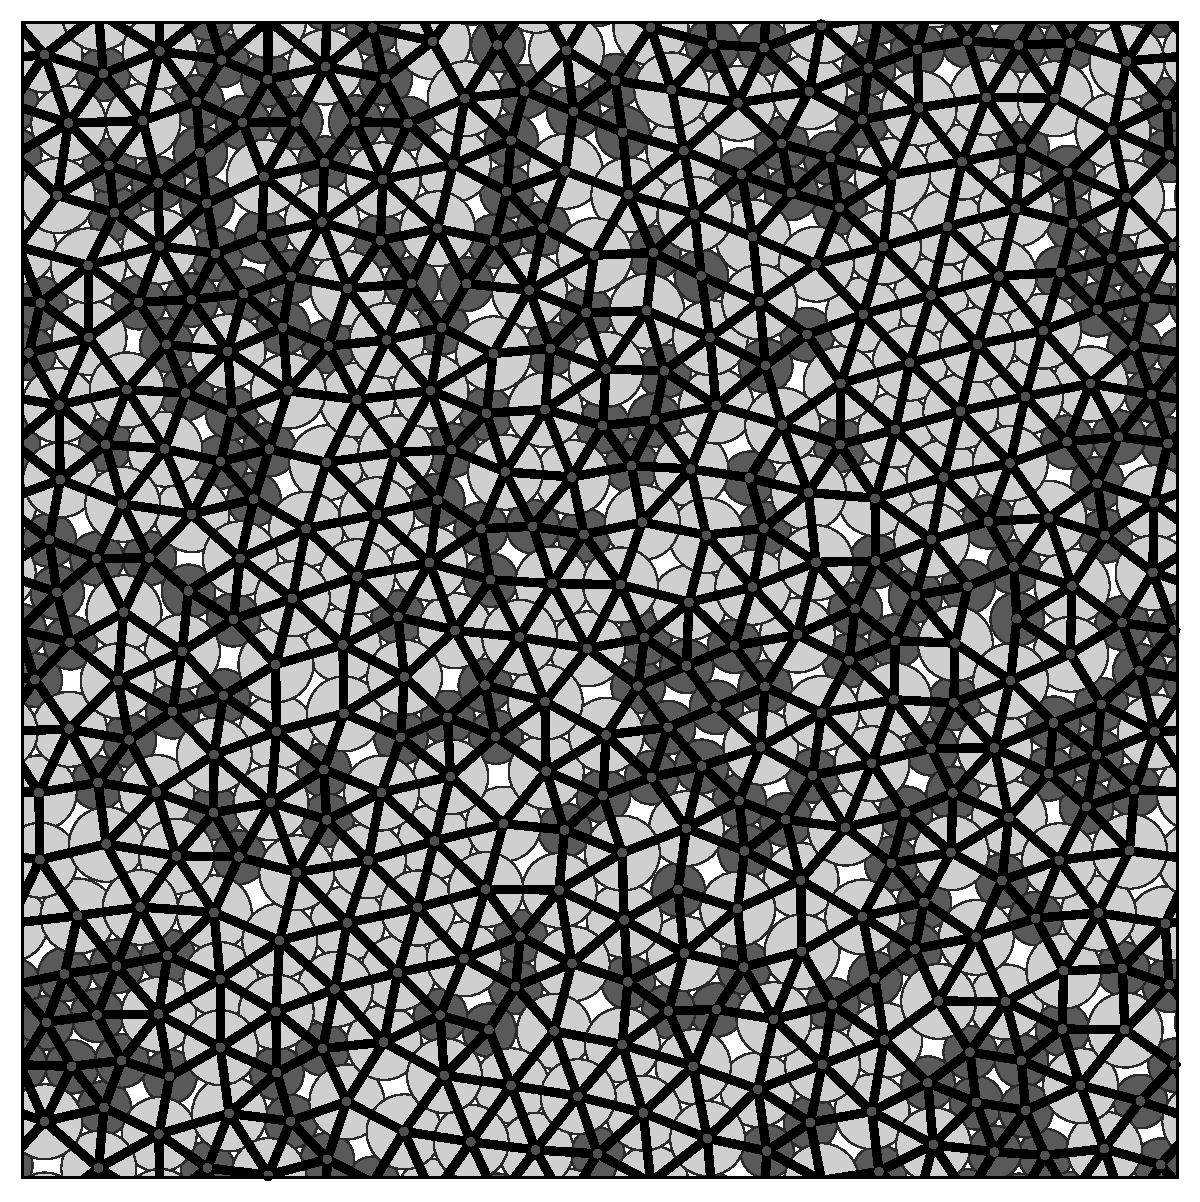
\includegraphics[width=.32\textwidth]{chapters/2-Background/Figures/Stacked.pdf}\hfill
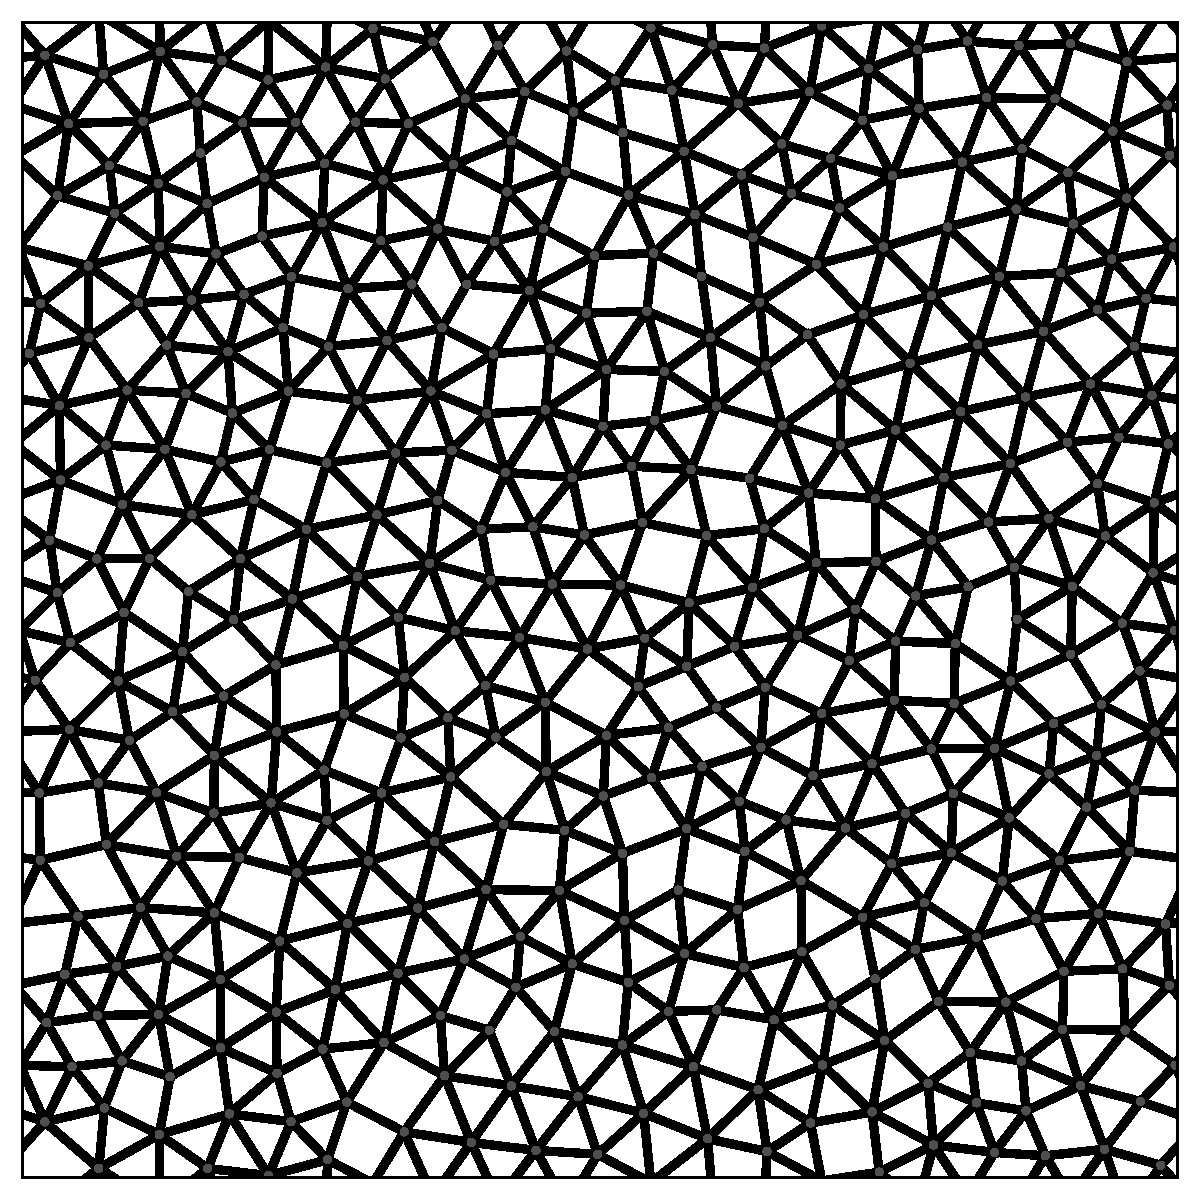
\includegraphics[width=.32\textwidth]{chapters/2-Background/Figures/network.pdf}
\caption[Steps for generating a packing-derived network from 400 soft spheres.]{
Steps for generating a packing-derived network from 400 soft spheres at $\phi = 1$.\newline 
\textbf{Left:} A bidisperse disk packing with a radius ratio of $1:1.4$ in an energy-minimised state. \newline
\textbf{Middle:} Network bonds defined from the contact network of overlapping spheres. \newline
\textbf{Right:} Disks removed, leaving only the bond and node of the network.}
\label{fig:SingleNetworkGeneration}
\end{figure}

Network bonds are constructed from the contact network of an equilibrated packing \cite{lerner_simulations_2013,ellenbroek_non-affine_2009,mangal_topological_2023}. A network node is placed at the centre of each disk. For every overlapping pair of disks, the corresponding nodes are connected by a bond whose natural length is given by their centre-to-centre distance in the energy-minimised configuration.

After all contacts have been processed, the disks themselves are removed, leaving a network composed solely of nodes and bonds. This construction procedure is illustrated in \cref{fig:SingleNetworkGeneration}. 

In this work, we take $\phi = 1 > \phi_J \approx 0.84$ unless stated otherwise \cite{chacko_slow_2019,ikeda_unified_2012}. For single networks, this corresponds to an average connectivity $z \approx 5.4$, which lies well above the isostatic threshold. In principle, networks with lower connectivity (while remaining above the isostatic threshold $z=4$) could be generated by preparing packings at $\phi$ closer to $\phi_J$. Instead, we obtain lower-connectivity networks by iteratively pruning bonds from an initially highly connected network constructed at $\phi=1$, following the procedure described below. This allows for tighter control of the network connectivity when studying systems with lower coordination.

These packing-derived networks provide a simple yet robust alternative to lattice-based networks. They exhibit emergent positional disorder, good numerical stability, and can be straightforwardly extended to three dimensions, as demonstrated in \cite{shivers_normal_2019, shivers_strain-controlled_2023, shivers_nonlinear_2020}. We therefore use them as the primary network structures considered in \cref{sec:Ultradelayed,sec:DoubleNetworks}.

\subsubsection{Pruning Networks} \label{sec:PrunningNetwork}
During network construction, the resulting graphs can contain disconnected clusters and dangling components (see \cref{fig:PruningNetworks}). These elements do not contribute to the static mechanical stress of the networkand are therefore removed before simulation.

Dangling components, shown in \cref{fig:PruningNetworks}a, consist of portions of the network attached to the bulk by a single bond. In graph theory, these correspond to biconnected components connected to the main network via a bridge edge. These are pruned by identifying bridge bonds and removing the associated dangling components. Disconnected clusters, illustrated in \cref{fig:PruningNetworks}b, are eliminated by identifying all connected components of the network and retaining only the largest component, which corresponds to the bulk network. To perform this analysis efficiently, we represent the network as an undirected graph, with bonds as edges, and use the \texttt{NetworkX} Python package \cite{SciPyProceedings_11} to identify connected components, biconnected components, and bridges.

\begin{figure}
    \centering
    \begin{subfigure}{0.45\linewidth}
        \centering
        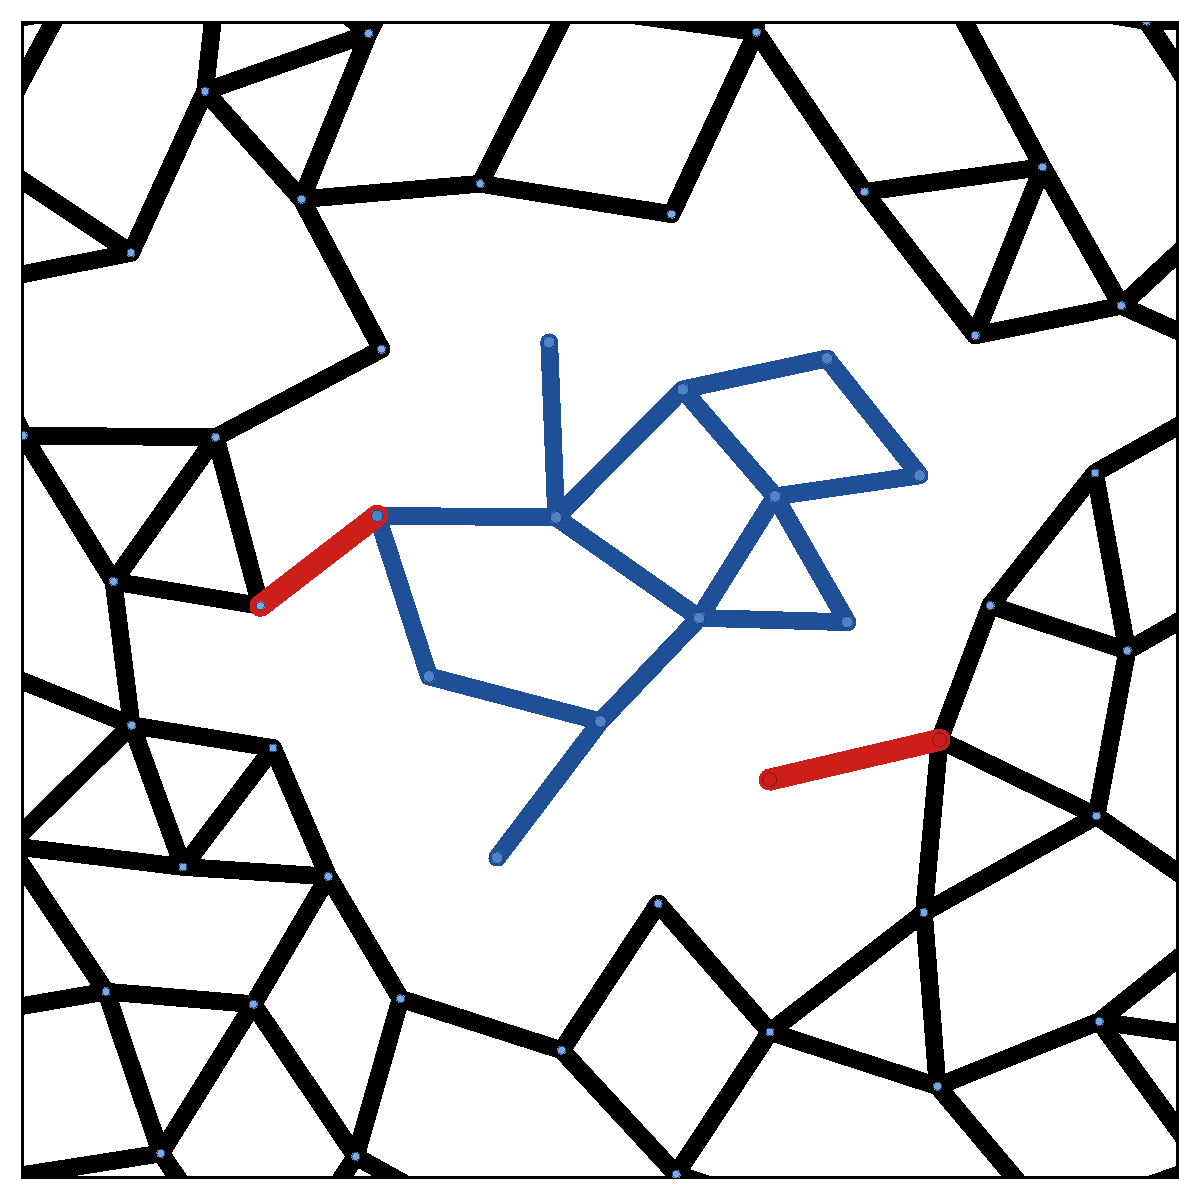
\includegraphics[width=\linewidth]{chapters/2-Background/Figures/network_dangling_motifs_400.pdf}
        \textbf{(a)}
    \end{subfigure}
    \begin{subfigure}{0.45\linewidth}
        \centering
        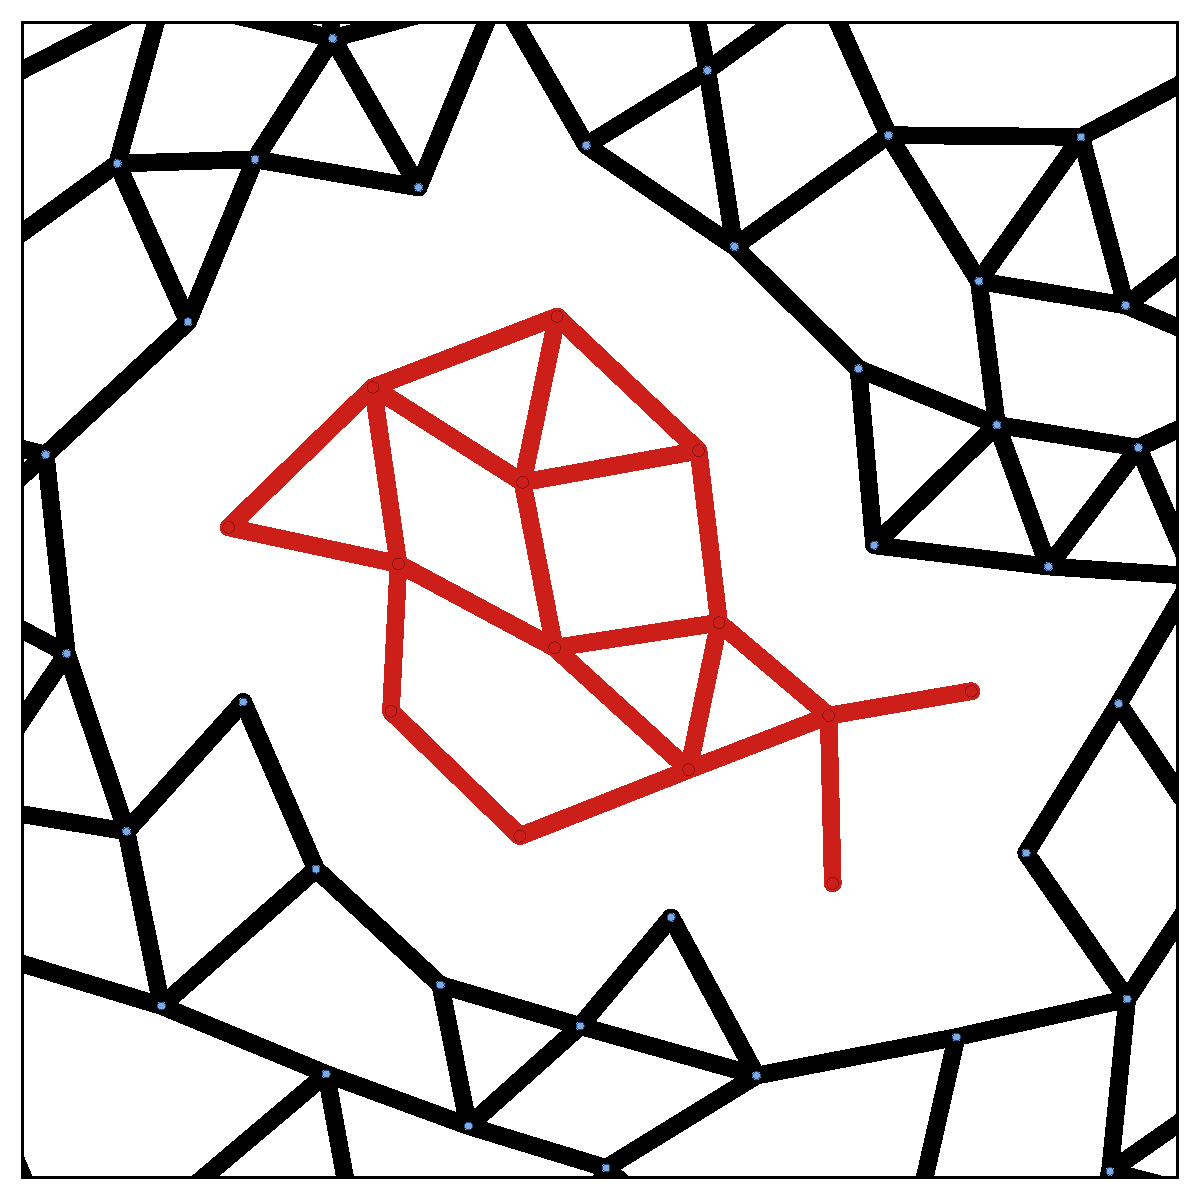
\includegraphics[width=\linewidth]{chapters/2-Background/Figures/network_disconnected_cluster_400.pdf}
        \textbf{(b)}
    \end{subfigure}
    \caption[Dangling and disconnected clusters.]{{\bf a)} A dangling cluster (blue) is defined as a cluster of bonds connected to the rest of the network by only one bond (a bridge, shown in red). These are detected and removed by removing bridges, i.e., bonds that disconnect the graph when cut. {\bf b)} A disconnected cluster (red) is a cluster of bonds that is disconnected from the bulk network. These are removed by identifying all connected components and retaining only the largest one.}
    \label{fig:PruningNetworks}
\end{figure}

Once a clean network has been generated, it can be pruned to reduce its average connectivity. This procedure is analogous to the bond dilution used in lattice-based networks to introduce disorder, although additional care is required due to the intrinsic positional disorder already present.

Bonds are removed selectively based on the local pair connectivity $z_{ij}=z_i+z_j$, where $z_i$ and $z_j$ denote the coordination numbers (i.e. the number of bonds) of the nodes connected by bond $(i,j)$. Bonds associated with the most highly connected node pairs are preferentially pruned to minimise spatial heterogeneity in the coordination field \cite{wyart_elasticity_2008, lerner_breakdown_2014}. This process is repeated until the target average connectivity is reached. Any dangling or disconnected components that emerge during pruning are identified and removed as they are created.

\subsection{Calculating Stress} \label{sec:virialStress}

The concept of stress has been discussed extensively throughout this thesis and derived within the framework of continuum mechanics (see \cref{sec:StressAndStrain,sec:StressTensor}). In molecular dynamics simulations, however, stress is defined in terms of the underlying discrete particle interactions.

In principle, the macroscopic stress can be obtained via the principle of virtual work by numerically differentiating the system Hamiltonian with respect to an imposed strain. While formally exact, this approach is computationally expensive, as the derivative is typically evaluated using finite differences. Consequently, each stress evaluation requires relaxing the system following a small strain increment.

Instead, molecular dynamics simulations typically report the virial stress tensor, which can be computed efficiently from the instantaneous particle forces and positions. While there are many formulations of the virial stress tensor \cite{walton_pressure_1983,erpenbeck_einstein-kubo-helfand_1995,tsai_virial_1979}, we will present a brief derivation of the virial stress tensor derived by Irving and Kirkwood in Ref.~\cite{irving_statistical_1950} in two dimensions.


Following the arguments of Doi and Edwards in Ref.~\cite{doi_theory_1988}, we consider an arbitrary line perpendicular to the $j$-axis, which intersects the network at a position $h$ along that axis. The $ij$ component of the stress across this line, $\sigma_{ij}(h)$, is defined as the $i$ component of the force (per unit length) exerted by the portion of the network above the line on the portion below it, which we denote by $F_i(h)$. The macroscopic stress $\Sigma_{ij}$ is then obtained by averaging $\sigma_{ij}(h)$ along the $j$-direction,
\begin{gather}
    \Sigma_{ij} = \langle \sigma_{ij}(h) \rangle = \frac{\langle F_i(h) \rangle}{L_i}, \\
    \Sigma_{ij} = \frac{1}{L_i L_j}\int_0^{L_j} F_i(h)\, dh,
    \label{eq:virialDevInt}
\end{gather}
where $L_i$ is the system length in the $i$ direction and $L_j$ is the extent of the averaging along the $j$-axis.  Their product $L_iL_j \equiv A$ is the system area. For simplicity, we neglect solvent contributions and retain only the contribution to the stress from the inter-node forces.
 
The force $F_i(h)$ can be written as the sum of the $i$-components of the pairwise forces $f_{mn}$ exerted on node $m$ by node $n$,
\begin{equation}
    F_i(h) = \sum_{m,n} f_{mn,i}\,
    \Theta(h-r_{n,j})\Theta(r_{m,j}-h),
    \label{eq:virialDevForce}
\end{equation}
where $r_{n,j}$ is the $j$-coordinate of node $n$. The two Heaviside functions restrict node $n$ to lie below the line and node $m$ above it. Substituting \cref{eq:virialDevForce} into \cref{eq:virialDevInt} and integrating over $h$ yields
\begin{subequations}
\begin{align}
    \Sigma_{ij}
    &= \frac{1}{A}\sum_{m,n}
    f_{mn,i}(r_{n,j}-r_{m,j})
    \Theta(r_{n,j}-r_{m,j})
    \label{eq:virialDevTheta} \\
    \Sigma_{ij} &= \frac{1}{2A}\sum_{m,n}
    f_{mn,i}(r_{n,j}-r_{m,j})
    \label{eq:virialDevfinal} \\
    \Sigma_{ij} &= \frac{1}{2A}\sum_{m,n}
    f_{mn,i}\, r_{mn,j},
    \label{eq:virialStress}
\end{align}
\end{subequations}
where $\bm{r}_{mn}=\bm{r}_n-\bm{r}_m$. The Heaviside factor in \cref{eq:virialDevTheta} selects pairs with $r_{n,j}>r_{m,j}$. Using Newton's third law, $\bm{f}_{mn}=-\bm{f}_{nm}$, and symmetry under exchange of $m$ and $n$, this restriction can be replaced by the factor of $1/2$, which corrects for double counting in the summation, as seen in \cref{eq:virialDevfinal,eq:virialStress}

The derivation above extends trivially to three dimensions, where instead force contributions above and below an arbitrary plane perpendicular to the $j$-axis are considered. Calculating the stress by this approach eliminates the computation of numerical derivatives and is more computationally efficient, as both $\bm{r}_{ij}$ and $\bm{f}_{ij}$ are already calculated at each timestep when evaluating the system's dynamics. A more thorough derivation of the virial stress tensor, including fluid effects, can be found in Ref.~\cite{yang_generalized_2012}.

\subsection{Generalised Lees--Edwards Boundary Conditions} \label{sec:Lees-Edwards}

When studying rheology, we aim to characterise a material's response to an imposed bulk stress or strain. In experimental settings, this is typically achieved by placing a sample of the material in a rheometer and imposing the desired loading or deformation through the motion of one or more boundaries. To ensure that the measured response reflects the bulk behaviour, samples are typically made sufficiently large that edge effects do not dominate the physics.

Achieving such system sizes in simulations, however, is often computationally prohibitive. A common strategy to mitigate this limitation is to employ periodic boundary conditions, whereby material leaving one side of the unit cell re-enters on the opposite side. This construction removes physical boundaries from the computational domain and thereby eliminates edge effects. Consequently, macroscopic strains must be imposed through alternative methods rather than via conventional boundary-driven forcing.

\begin{figure}[b]
    \centering
    \begin{subfigure}[t]{0.5\linewidth}
        \centering
        \includegraphics[width=.8\linewidth]{chapters/2-Background/Figures/TriClinic.tikz}
        \caption{Triclinic Boundary Conditions}
        \label{fig:Tri-Clinic}
    \end{subfigure}%
    \hfill
    \begin{subfigure}[t]{0.5\linewidth}
        \centering
        \includegraphics[width=.8\linewidth]{chapters/2-Background/Figures/LeesEdwards.tikz}
        \caption{Lees Edwards Boundary Conditions}
        \label{fig:Lees-Edwards}
    \end{subfigure}
    \caption{An Illustration of two equivalent boundary conditions used in simulations to apply macroscopic stresses to a system} 
    \label{fig:BoundaryConditions}
\end{figure}

In periodic simulations, macroscopic deformation is imposed by modifying the lattice vectors, which define the mapping between the unit cell and its periodic images. Simple loading protocols can therefore be implemented by appropriately deforming the simulation box and its lattice vectors, as illustrated in \cref{fig:Tri-Clinic}. This approach is commonly referred to as the use of triclinic boundary conditions, with the terminology derived from the triclinic crystal lattice.

While this method permits arbitrary homogeneous deformations, it can be computationally costly in practice due to the need to transform between bases when evaluating minimum-image distances. Moreover, at large strains, the unit cell can become highly skewed, which may lead to numerical inefficiencies. To address these issues, Lees and Edwards proposed a modified set of periodic boundary conditions that achieves the same macroscopic shear while remaining computationally efficient \cite{lees_computer_1972}.

To impose shear in the $x$ direction using Lees--Edwards boundary conditions, particle positions $\mathbf{r}_i=(x_i,y_i)$ are affinely transformed according to
\begin{equation}
    \begin{pmatrix}x_i \\ y_i
    \end{pmatrix} \to 
    \begin{pmatrix}x_i + \gamma y_i \\ y_i
    \end{pmatrix}
\end{equation}
whilst periodic images are shifted by an amount $\gamma L_y$ between adjacent rows, as shown in \cref{fig:Lees-Edwards}. This construction is computationally advantageous because the primary simulation cell remains orthogonal. Implementation details can be found in Ref.~\cite{allen_computer_2017}.

\section{Conclusion}
% \red{
    In this chapter, we have introduced the theoretical framework used throughout the remainder of this thesis. We began with a continuum description of stress and strain, establishing the tensorial quantities used to characterise deformation and internal forces, and introduced the linear elastic constitutive relation that serves as a reference point for identifying yielding, plasticity, and fracture. We also outlined the strain-controlled deformation protocols used in later chapters, namely oscillatory strain, step strain, and strain startup, each of which probes a different aspect of material response.
    
    We then considered force balance in the Stokes limit, which provides the appropriate description for the overdamped systems studied here. Within this framework, local irreversible rearrangements may be represented through a plastic eigenstrain, and the resulting redistribution of stress is described by the Oseen tensor and the Eshelby stress propagator. These results provide the continuum basis for understanding how local events perturb the surrounding material and contribute to the bulk response.
    
    Finally, we introduced soft networks as model systems in which the coupling between structure, deformation, and failure can be resolved explicitly. We described the mechanics of semi-flexible filaments, the overdamped dynamics used to evolve the network, and the different notions of rigidity relevant to disordered systems. We then discussed how fracture emerges through heterogeneous stress concentration, non-affine rearrangements, and bond breakage, and introduced the network architectures and numerical methods used in later chapters, including lattice-based and packing-derived networks, pruning procedures, the virial stress tensor, and Lees--Edwards boundary conditions. Together, these concepts provide the basis for the analysis of damage accumulation under cyclic loading, delayed yielding following an imposed step strain, and stress redistribution and toughening in double-network materials.
% }

\section{Units and Parameters}
We will work in units throughout this thesis where $\zeta=1$.
Need to define the parameters used in the simulations for timestepping.

\newpage
\begin{subappendices}
    % !TeX root = ../../thesis.tex
\section{Fourier Derivation of the Oseen Tensor}
\label{app:OseenDerivation}

This appendix provides the intermediate derivation for the results quoted in \cref{sec:Oseen}. Starting from the Stokes equations for a plastic eigenstrain field,
\begin{subequations}
\label{eq:AppStokes}
\begin{align}
- \nabla p(\bm{r}) + \mu \nabla^2 \bm{u}(\bm{r}) &= 2\mu \nabla \cdot \bm{\epsilon}^{\mathrm{pl}}(\bm{r}), \\
\nabla \cdot \bm{u} &= 0,
\end{align}
\end{subequations}
Applying the Fourier transform to \cref{eq:AppStokes} gives
\begin{equation}
- i k_i \hat{p} - \mu k^2 \hat{u}_i = 2\mu i k_j \hat{\epsilon}_{ij}^{\mathrm{pl}}.
\label{eq:AppStokesFourier}
\end{equation}

Using incompressibility in Fourier space,
\[
    k_i\hat{u}_i = 0,
\]
and multiplying \cref{eq:AppStokesFourier} by $k_i$, we obtain
\begin{equation}
    \hat{p} = -2\mu \frac{k_i k_j}{k^2}\hat{\epsilon}_{ij}^{\mathrm{pl}}.
    \label{eq:AppPressureKernel}
\end{equation}
Substituting into \cref{eq:AppStokesFourier} gives
\begin{equation}
    \hat{u}_i = -\frac{2i}{k^2}\left(\delta_{ij} - \frac{k_i k_j}{k^2}\right)k_l \hat{\epsilon}_{jl}^{\mathrm{pl}}.
\end{equation}
Recognising the transverse projector then gives the Oseen tensor
\begin{equation}
    \hat{\mathbb{O}}_{ij} = \frac{1}{\mu k^2}\left(\delta_{ij} - \frac{k_i k_j}{k^2}\right),
    \label{eq:AppOseen}
\end{equation}
which matches \cref{eq:Oseen}.

Hence,
\begin{equation}
    \hat{u}_i = -2\mu \hat{\mathbb{O}}_{ij} i k_l \hat{\epsilon}_{jl}^{\mathrm{pl}},
\end{equation}
and
\begin{equation}
    i k_m \hat{u}_i = 2\mu k_m \hat{\mathbb{O}}_{ij} k_l \hat{\epsilon}_{jl}^{\mathrm{pl}},
\end{equation}
which are the Fourier-space displacement and deformation-gradient fields used in \cref{sec:EshelbyPropogator}.

\end{subappendices}
